\documentclass[journal]{IEEEtran}

\usepackage{graphicx}
\usepackage{amsmath}
\usepackage{amssymb}
\usepackage{mathtools}
\usepackage{array}
\usepackage{multirow}


\ifCLASSOPTIONcompsoc
  \usepackage[caption=false,font=normalsize,labelfont=sf,textfont=sf]{subfig}
\else
  \usepackage[caption=false,font=footnotesize]{subfig}
\fi


\def\*#1{\bar{#1}} % an abbreviation of \bar{}

\graphicspath{{figures/}}

% correct bad hyphenation here
\hyphenation{op-tical net-works semi-conduc-tor}

\begin{document}

%\title{Design Solution for a Stephenson II Timed Path Generator and Application to Robot Limb Design}

%\title{Computational Timed Path Generation for the Synthesis of Dynamic Behavior}

\title{Computational Six-bar Synthesis for Implementing Dynamic Behavior}

\title{Root-Finding for Linkage Design and Dynamic Behavior}

\title{Root-Finding for the Design of Linkage Systems with a Dynamic Behavior}

\title{Root Finding for Linkage Designs with Prescribed Dynamic Behavior}

\title{Root Finding for Linkage Designs with Prescribed Energetic Response during Dynamic Loading}

\title{Computational Kinematic Synthesis for Dynamic Behaviors}


\title{Large Scale Root Finding for Designing Mechanisms with Prescribed Dynamic Behavior}

\title{Endowing Mechanisms with Dynamic Behaviors Through Large Scale Root Finding}

\title{Large Scale Root Finding for the Kinematic Design of Mechanisms with Prescribed Dynamic Behavior}



\author{Mark~M.~Plecnik %,~\IEEEmembership{Member,~IEEE,}
        and~Ronald~S.~Fearing,~\IEEEmembership{Member,~IEEE}% <-this % stops a space
\thanks{M.~Plecnik is a postdoctoral scholar in the Biomimetic Millisystems Lab at the University of California, Berkeley, CA, 94720 USA e-mail: {\tt\small mplecnik@berkeley.edu}}% <-this % stops a space
\thanks{R.~S.~Fearing is director of the Biomimetic Millisystems Lab and a professor in the Department of Electrical Engineering \& Computer Science, University of California, Berkeley, CA, 94720 USA e-mail: {\tt\small ronf@eecs.berkeley.edu}}% <-this % stops a space
\thanks{Manuscript received November xx, 2018; revised Month xx, 20xx.}}

% The paper headers
\markboth{IEEE Transactions on Robotics,~Vol.~xx, No.~xx, Month~20xx}%
{Plecnik and Fearing: Design Solution for a Stephenson II Timed Path Generator}

\maketitle

\begin{abstract}
The abstract goes here.
\end{abstract}

\begin{IEEEkeywords}
IEEE, IEEEtran, journal, \LaTeX, paper, template.
\end{IEEEkeywords}

% For peerreview papers, this IEEEtran command inserts a page break and
% creates the second title. It will be ignored for other modes.
\IEEEpeerreviewmaketitle


\section{Introduction}
\label{sec:intro}
% The very first letter is a 2 line initial drop letter followed
% by the rest of the first word in caps.
% 
% form to use if the first word consists of a single letter:
% \IEEEPARstart{A}{demo} file is ....
% 
% form to use if you need the single drop letter followed by
% normal text (unknown if ever used by the IEEE):
% \IEEEPARstart{A}{}demo file is ....
% 
% Some journals put the first two words in caps:
% \IEEEPARstart{T}{his demo} file is ....
% 
% Here we have the typical use of a "T" for an initial drop letter
% and "HIS" in caps to complete the first word.
\IEEEPARstart{T}{here} are no simple tools for designing dynamic machines.
The leading approaches are based in optimization and intuition.
We demonstrate a method that excludes the former and lessens dependence on the latter.
This work is enabled by a new algorithm in numerical homotopy continuation that can find nearly complete solution sets of highly nonlinear systems of equations.
%
The connection to design occurs as these systems of equations comprise of geometric design constraints, and their variables are design parameters.
Rather than search through the design space for a set of parameters that satisfy all constraints and minimize some objective, design constraints are posed as systems with isolated roots, where gathering roots is equivalent to compiling candidate design parameters.  The result is a thorough exploration of the design space.


Specifically, we care to design machines consisting of rigid links and springs that perform some specified motion when subjected to expected loads.
We narrow the scope of expected loads by considering only actuator torque (input) and the force acting on an end effector point (output), see Fig. \ref{intro_sixbar}.
The time-varying magnitudes of this force and torque define inertial motion, but their ratio (called mechanical advantage) is purely geometric\footnote{Neglecting losses}, connecting kinematic constraints to dynamic behavior.

Despite its geometric nature, mechanical advantage may be posed to take a variety of forms prior to searching for an instantiating geometry.
These forms may be grouped with inertial and force elements (masses, motors, springs), then simulated to acquire the resulting dynamics.
In this way, configuration-dependent mechanical advantage curves that create a desired dynamic response may be found beforehand in order to serve as a design goal for kinematic synthesis.


\begin{figure}[!t]
\centering
\subfloat[]{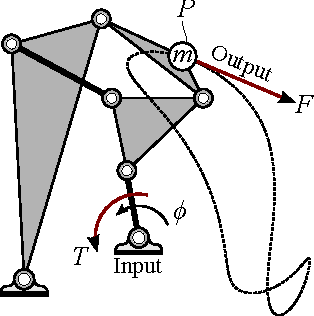
\includegraphics[scale=0.7]{intro_sixbar_a}%
\label{intro_sixbar_a}}
\hfil
\subfloat[]{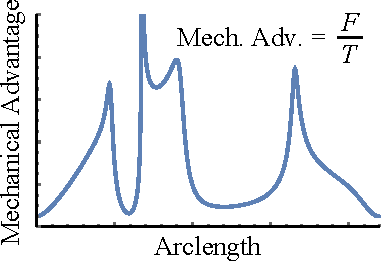
\includegraphics[scale=0.6]{intro_sixbar_b}%
\label{intro_sixbar_b}}
\caption{A six-bar linkage transforms input torque to output force in a highly nonlinear way.}
\label{intro_sixbar}
\end{figure}




To find an instantiating geometry for a desired mechanical advantage form requires investigation of a sufficiently complex design space capable of satisfying our customization needs.
%Furthermore, configuration-based mechanical advantage must be design simultaneously with desired mechanism configurations.
Luckily, we do not need to consider overly complicated mechanism topologies.
For example, a six-bar linkage, shown in Fig. \ref{intro_sixbar}, is a single degree-of-freedom mechanism.
Despite its simple structure, it is capable of producing complex, constrained motions e.g. it may draw a degree 16 plane curve \cite{primroseSixbarMotionII1967}.
On the other hand, this same simple structure begets challenging nonlinearities within six-bar design equations e.g. the equations investigated in this work are of degree $8.8 \times 10^{12}$.
%On the other hand, despite its simple structure, the design equations associated with six-bar linkages are challenging due to vast nonlinearities in their structure e.g. the equations investigated in this work are of degree xx.
To corral this daunting number, we implement the Finite Root Generation technique \cite{plecnikFindingOnlyFinite2017}, based in numerical homotopy continuation.
This technique estimated the number of finite roots of this system to be around $1.5 \times 10^6$, and found these roots for a numerically general version of the system.
This set of roots itself is a new design instrument, which can be used repeatedly in conjunction with another well established continuation technique \cite{morganCoefficientparameterPolynomialContinuation1989} to efficiently solve systems of this structure.
The equations themselves comprise of the kinematic constraints to coordinate endpoint $P$ with angle $\phi$ of a Stephenson II six-bar linkage, see Fig. \ref{intro_sixbar}.
The complete solution of these equations is first presented in this work.
This solution is particularly useful for synthesizing a point path to coordinate with the mechanical advantage of an input link, albeit indirectly.


To illustrate our approach and demonstrate its utility for designing a machine with some desired dynamic behavior, 
%we present a running example related to legged locomotion.
we design a leg mechanism suitable for a small running robot.
The mechanism is powered by a series-elastic actuator, with mechanical advantage specified in order to deliver kinetic energy during push-off at powers greater than its motor's output.
This behavior is termed power modulation \cite{haldaneRoboticVerticalJumping2016}.
In addition to achieving the required mechanical advantage, we design a foot path that recycles the leg each step with the motor running only in the forward direction.
In a related work \cite{plecnikAdjustablePowerModulation2019}, this mechanism was prototyped and tested.



\section{Literature Review}
\label{sec:lit_rev}

\subsection{Mechanism Synthesis}
\label{sec:mech_synth}

Previous design methods that produce dynamic characteristics in mechanisms focus on reducing the shaking forces and moments that act on the fixed frame, or reducing fluctuations in actuator torque.
Berkof, Tepper, and Lowen \cite{berkofNewMethodCompletely1969,tepperGeneralTheoremsConcerning1972,lowenBalancingLinkagesUpdate1983} formulated conditions for fixing the center of mass of a moving linkage, which removes the shaking force during dynamic operation at any speed.
Skreiner \cite{skreinerDynamicAnalysisUsed1970} demonstrated how to reduce speed fluctuations and pin forces by adding a spring to a four-bar.
Conte et al. \cite{conteOptimumMechanismDesign1975} included kinetostatic force equations at a sampling of configurations for a four-bar linkage with prescribed motion in order to compute optimal dimensions that minimize shaking forces/moments, bearing forces, or input torques.
Yao and Yan \cite{yaoNewMethodTorque2003} use non-circular gears to reduce fluctuations in driving torque for planar linkages.
Yan and Yan \cite{yanIntegratedControlMechanism2009} present a comprehensive optimization procedure for the design of four-bar linkages that satisfies kinematic requirements while reducing shaking force/moment and motor power dissipation.  They consider link dimensions, mass, input speed trajectory, and servomotor control parameters as design variables.
Moore et al. \cite{mooreDeterminationCompleteSet2009} computed the complete set of force and moment balanced four-bars.


A few approaches more explicitly deal with time and motion specifications.  
Sherwood \cite{sherwoodDynamicSynthesisMechanism1968} and Liniecki \cite{linieckiSynthesisSlidercrankMechanism1970} designed slider-crank mechanisms that achieve desired positions and velocities coordinated in time by modifying dimensions between numerical dynamic computations.
Halter and Carson \cite{halterMechanismForceSystemSynthesis1975} developed a design procedure to add mechanical elements to an existing mechanism in order to obtain a desired motion-time response.  Desired generalized forces of to-be-synthesized mechanical elements were computed from inverse dynamics calculations.  Design parameters of these mechanical elements were then computed through optimization as a curve fitting problem to the desired generalized forces.  Zhen \cite{zhenAnalyticalSynthesisSpring1988} applied dynamic spring synthesis to spatial mechanisms.


Starr \cite{starrDynamicSynthesisConstraint1973} considered not just how to implement desired dynamic motions, but how to specify those motions using optimal control theory.  
Later, Manoochehri and Seireg \cite{manoochehriComputerBasedMethodologyForm1990} also employed these optimal control techniques.  Chen and Tsai \cite{chenKinematicDynamicSynthesis1993} discussed how to design gearing for a manipulator to possess both kinematic isotropy and good acceleration capacity.


Another dynamic consideration is the presence of vibrations in high speed machinery.  
Matthew and Tesar \cite{matthewCamSystemDesign1976} considered the effects of vibrations and inertial forces on cam design.
Li and Kota \cite{liDynamicAnalysisCompliant2002} analyzed the frequency response of a micro machined stroke amplifying mechanism for an electrostatic actuator and conducted sensitivity analyses useful for synthesis.
Motivated by their investigation of parallel manipulators, Martini et al. \cite{martiniElastodynamicBehaviorBalanced2014} study mass balanced and elastically compensated closed chains through the addition of weights and springs.
Design methods that consider the kineto-elastodynamic effects in mechanisms were presented by Imam and Sandor \cite{imamHighSpeedMechanismDesign1975}.
Tantanawat and Kota \cite{tantanawatDesignCompliantMechanisms2007} investigated the benefits of strain energy storage in the dynamic performance of a compliant flapping mechanism.



%A motivation for this work is mechanism design for dynamic mobile robots.
%
%
%Applications to mobile robots have lead
%
%This work is partially motivated by interest in dynamic mobile robots
%
%
%The design of dynamic mobile robots has indicated various principles conducive to successful locomotion.


\subsection{Legged Robots}
\label{sec:leg_rob}


One motivation for this work is to design dynamic machines suitable for legged robots.
The literature indicates various design principles and outstanding challenges to direct the formulation of design requirements.
With respect to small hexapedal running robots, Clark et al. \cite{clarkBiomimeticDesignFabrication2001} and Hoover et al. \cite{hooverBioinspiredDesignDynamic2010} indicate the importance of passive mechanics, self-stabilization, open-loop/feedforward control, minimal actuation, and integrated manufacturing techniques in order to negotiate the strict limits on power, computation, and weight associated with of small robots.
Zarrouk et al. \cite{zarroukDynamicLeggedLocomotion2015} addressed the need of high speed turning in a hexapedal runner by taking advantage of dynamic roll and pitch instabilities.
The challenges of legged robots listed by Buehler \cite{buehlerDynamicLocomotionOne2002} include underactuated dynamics, friction limited horizontal ground forces, short stance times to apply control, bandwidth limitations, and limited power/energy densities of commercial actuators.
Collins et al. \cite{collinsEfficientBipedalRobots2005} leveraged passive-dynamics to create robots that mimic human walking with simple actuators that do not require precise joint-angle control.
Curran et al. \cite{curranDesignSeriesElasticActuators2008} indicated the role of series-elastic actuation in decoupling the limits of a DC motor from a dynamic task.
Semini et al. \cite{seminiDesignHyQHydraulically2011} stress the importance of high powered actuators.
In the analysis of a symmetric five-bar linkage, Kenneally and Koditschek \cite{kenneallyLegDesignEnergy2015} measured performance according to the conversion of battery energy into body energy, the minimization of touchdown losses, and the storing/return of energy during stance.
Blackman et al. \cite{blackmanLegDesignRunning2017} extended their analysis, highlighting the ability of this symmetric five-bar to achieve greater speeds and stability in one configuration, but greater jump height in another.
Brown et al. \cite{brownDesignMethodologyLinkage2017} analyzed the ability of this five-bar and other linkage designs to balance workloads between motors.
Kalouche \cite{kaloucheGOATLeggedRobot2017} designed a spatial linkage based on this five-bar.
Wensing et al. \cite{wensingProprioceptiveActuatorDesign2017} demonstrated the importance of torque density, high-bandwidth force control, and impact mitigation in quadrupedal running robots.



%% % %
%Clark et al. \cite{clarkBiomimeticDesignFabrication2001} built Sprawlita based on biological design principles extracted from studies on cockroach locomotion.  They indicate the importance of a stabilizing posture, a thrusting/stabilizing leg, passive visco-elastic structures, open-loop/feedforward control, and integrated construction.
%
%% % %
%In designing small dynamic robots, Hoover et al. \cite{hooverBioinspiredDesignDynamic2010} negotiated strict limits on power, computation, and weight by designing passive mechanical controls capable of self-stabilization.
%
%% % %
%Zarrouk et al. \cite{zarroukDynamicLeggedLocomotion2015} addressed roll and pitch instabilities for use in high speed turning in a minimally actuated hexapedal running robot.
%
%
%% % %
%Buehler \cite{buehlerDynamicLocomotionOne2002} details many of the challenges of legged robots including underactuated dynamics, friction limited horizontal ground forces, short stance times to apply control, bandwidth limitations, and limited power/energy densities of commercial actuators.
%
%% % %
%Collins et al. \cite{collinsEfficientBipedalRobots2005} designed passive-dynamic machines that mimic human walking without precise joint-angle control.  Compared to human muscle, they note that this control would require actuators of greater energetic output, more precision, and higher frequency response.
%
%% % %
%Curran et al. \cite{curranDesignSeriesElasticActuators2008} demonstrated the ability of a series-elastic actuator to decouple the limits of a DC motor from a dynamic task.
%
%% % %
%Semini et al. \cite{seminiDesignHyQHydraulically2011} chose a combination of hydraulic and electric actuators for their quadrupedal robot in order to achieve high powered motions.
%
%% % %
%Kenneally and Koditschek \cite{kenneallyLegDesignEnergy2015} chose a symmetric five-bar leg and measured its performance according to its ability to transduce battery energy into body energy, minimize touchdown losses, and store and return energy during stance.
%
%% % %
%Blackman et al. \cite{blackmanLegDesignRunning2017} extended their analysis of this five-bar, noting its ability to achieve greater speeds and stability in its ``knee down'' configuration, but greater jump heights from its ``knee up'' configuration.
%
%% % %
%Brown et al. \cite{brownDesignMethodologyLinkage2017} analyzed this five-bar alongside other linkage designs to balance the workload between motors.
%
%% % %
%Kalouche \cite{kaloucheGOATLeggedRobot2017} designed a spatial linkage based on this five-bar.
%
%% % %
%Wensing et al. \cite{wensingProprioceptiveActuatorDesign2017} indicate torque density, high-bandwidth force control, and impact mitigation as keys to success in the MIT Cheetah leg.
%

\subsection{Homotopy Continuation}
\label{sec:homotopy}

The role of homotopy continuation methods in mechanism design traces back to Roth and Freudenstein's bootstrap method \cite{rothSynthesisPathGeneratingMechanisms1963}. %
After that, more general methods focused on constructing homotopy paths absent of turning points or intersections \cite{zangwillPathwaysSolutionsFixed1981}, handling infinite roots by tracking in projective spaces \cite{wrightFindingAllSolutions1985}, and computing singular endpoints \cite{morganPowerSeriesMethod1992}. %
Additionally, researchers were interested in increasing the efficiency of computing large root sets by limiting the number of homotopy paths that need to be tracked. %
The work of Morgan and Sommese \cite{morganHomotopySolvingGeneral1987} lead to \emph{multihomogeneous homotopies} that take advantage of sparse monomial structures.  Variables are split into groups that define a factored start system of fewer roots, reducing the number of homotopy paths to track. %
Generalizations of this work lead to partitioned linear product homotopy \cite{verscheldeGBQAlgorithmConstructing1993,wiseAlgorithm801POLSYS2000}, general linear product homotopy \cite{verscheldeSymbolicHomotopyConstruction1993,verscheldeAlgorithm795PHCpack1999,suAlgorithm857POLSYS2006}, and polyhedral homotopy \cite{verscheldeHomotopiesExploitingNewton1994}. %
Hauenstein et al. \cite{hauensteinRegenerationHomotopiesSolving2011} introduced regeneration homotopy, an efficient method that exploits the sparse monomial structure of a system one equation at a time to find all of its isolated solutions. %
Plecnik and Fearing \cite{plecnikFindingOnlyFinite2017,plecnikStudyFindingFinite2017} introduced the Finite Root Generation method for solving mechanism synthesis equations.  
This is the solution technique used in this paper.  It institutes a stochastic procedure for generating startpoints that always track to finite roots.



In this work, we create a design procedure for instantiating dynamic behavior into a machine by applying FRG to obtain the complete solution of previously unsolved six-bar synthesis equations.
The process begins by posing a simplified system, referred to as a dynamic mock-up, that captures the desired dynamics, presented in Section \ref{sec:dynamic_mock-up}.
The mock-up indicates geometric constraints which are encoded into relevant synthesis equations, presented in Section \ref{sec:synth_eq}.
The FRG method was applied to solve these equations, presented in Section \ref{sec:frg}.
The roots obtained from this solution serve as an instrument to efficiently re-solve the synthesis equations for different geometric requirements.
We demonstrate this in Section \ref{sec:leg_app} by applying the results of FRG to the design of a leg mechanism that modulates power beyond its motors output during a fully rotatable running motion.



\section{Dynamic Mock-Up}
\label{sec:dynamic_mock-up}

To begin, we consider the dynamics of the mock-up system illustrated in Fig. \ref{dynamic_model}.
A motor twists a series spring, transmitting torque $T$ to an input crank.
This torque is transformed by the mechanical advantage of a to-be-designed linkage into a force $F_t$ at an end effector point that is resisted by an attached mass $m$ and in contact with a sliding mass $M$.
The direction of $F_t$ lies tangent to a point path $\mathcal{C}$ constrained by the to-be-designed linkage.


\begin{figure}[!t]
\centering
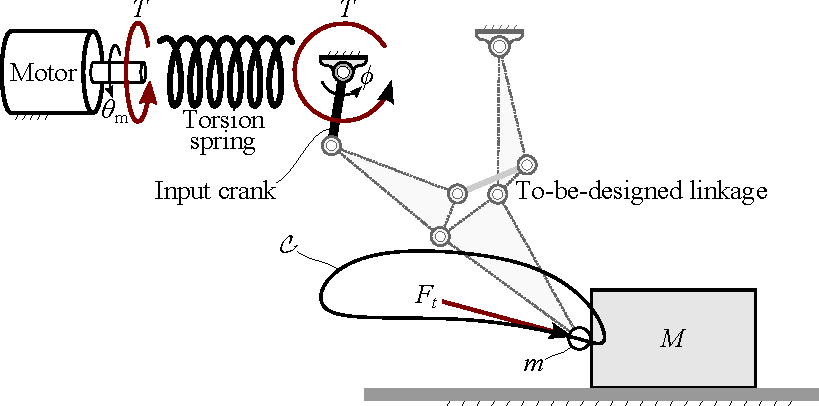
\includegraphics[width=1\linewidth]{dynamic_model}
\caption{A mock-up dynamic system used to inform desirable kinematic properties of a to-be-designed linkage.  The fixed motor is connected in series with a spring to an input crank.  Without any linkage existing yet, a user defined angle-arclength relationship describes how torques at the crank transform to forces at the masses.}
\label{dynamic_model}
\end{figure}


\subsection{Specifying Mechanism Characteristics}
\label{sec:spec_mech_char}

Although this to-be-designed linkage does not yet exist, we may freely specify its would-be characteristics.  
In particular, we specify its constrained point path and variable mechanical advantage as a function of the point's position along this path.
We accomplish this by clicking points on a computer screen, and interpolating curves through these points.
We choose the Fourier-based interpolation method used in \cite{plecnikControllingMovementTRR2016} to create periodic curves that are smooth everywhere.

\begin{figure}[!t]
\centering
\subfloat[]{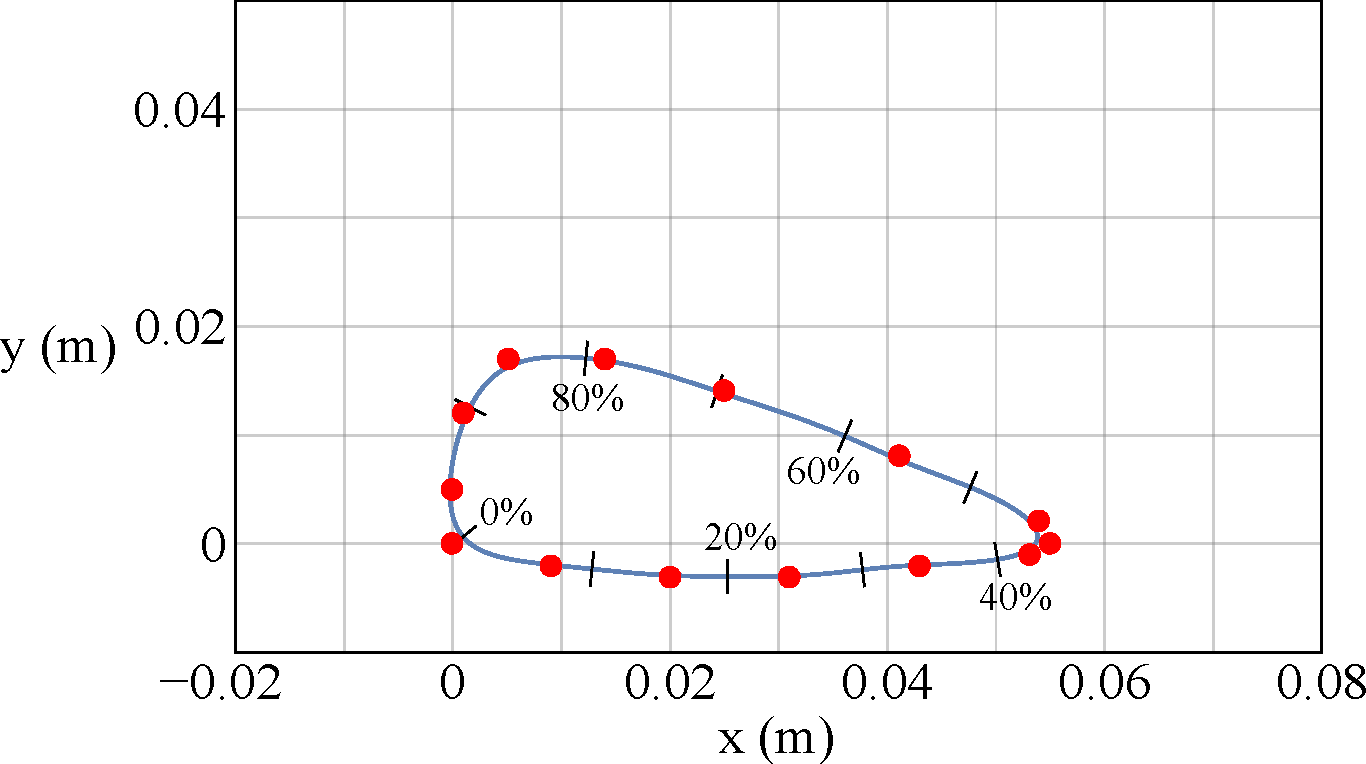
\includegraphics[scale=0.3]{clickspec_path}%
\label{clickspec_path}}
\hfil
\subfloat[]{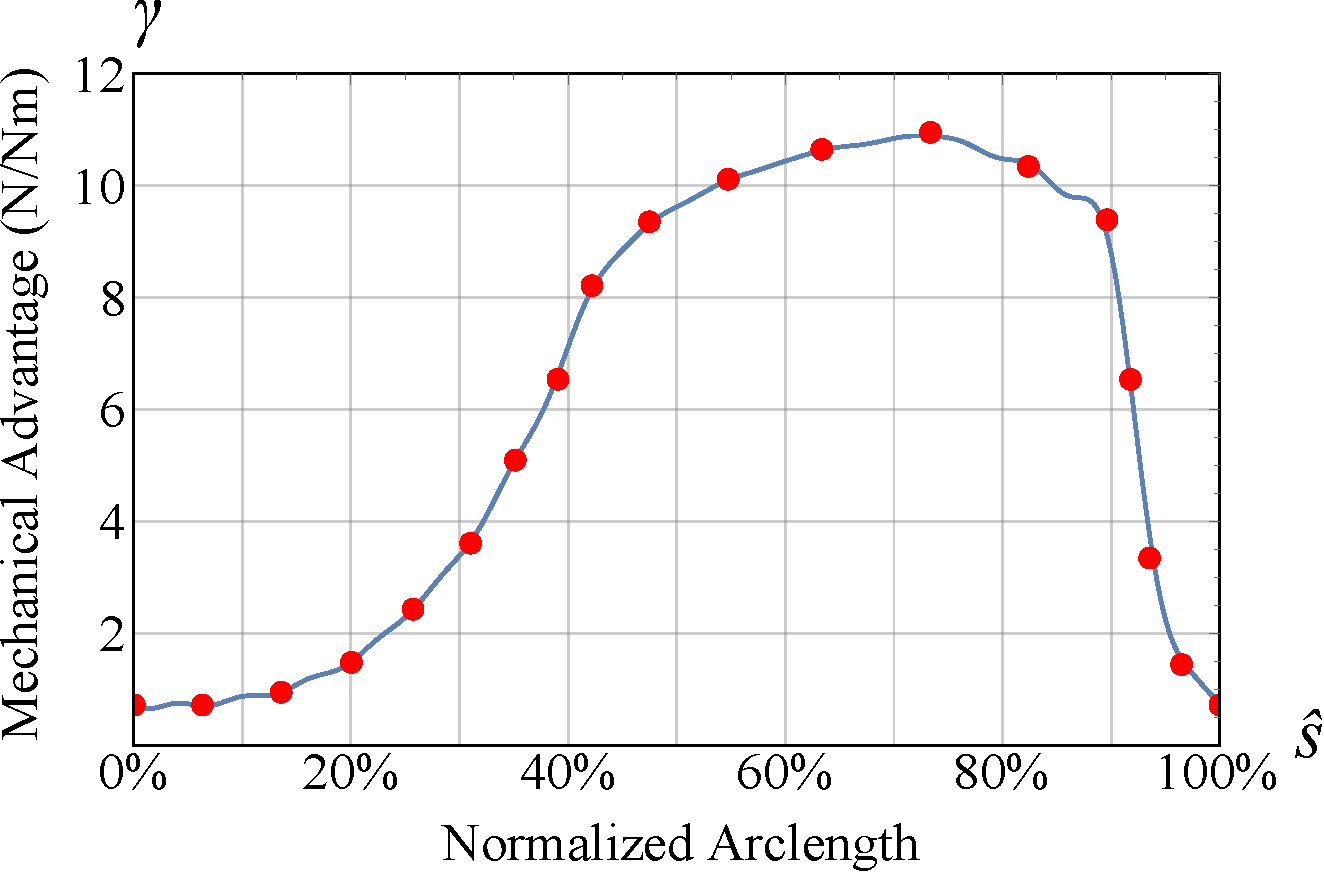
\includegraphics[scale=0.3]{clickspec_ma}%
\label{clickspec_ma}}
\hfil
\subfloat[]{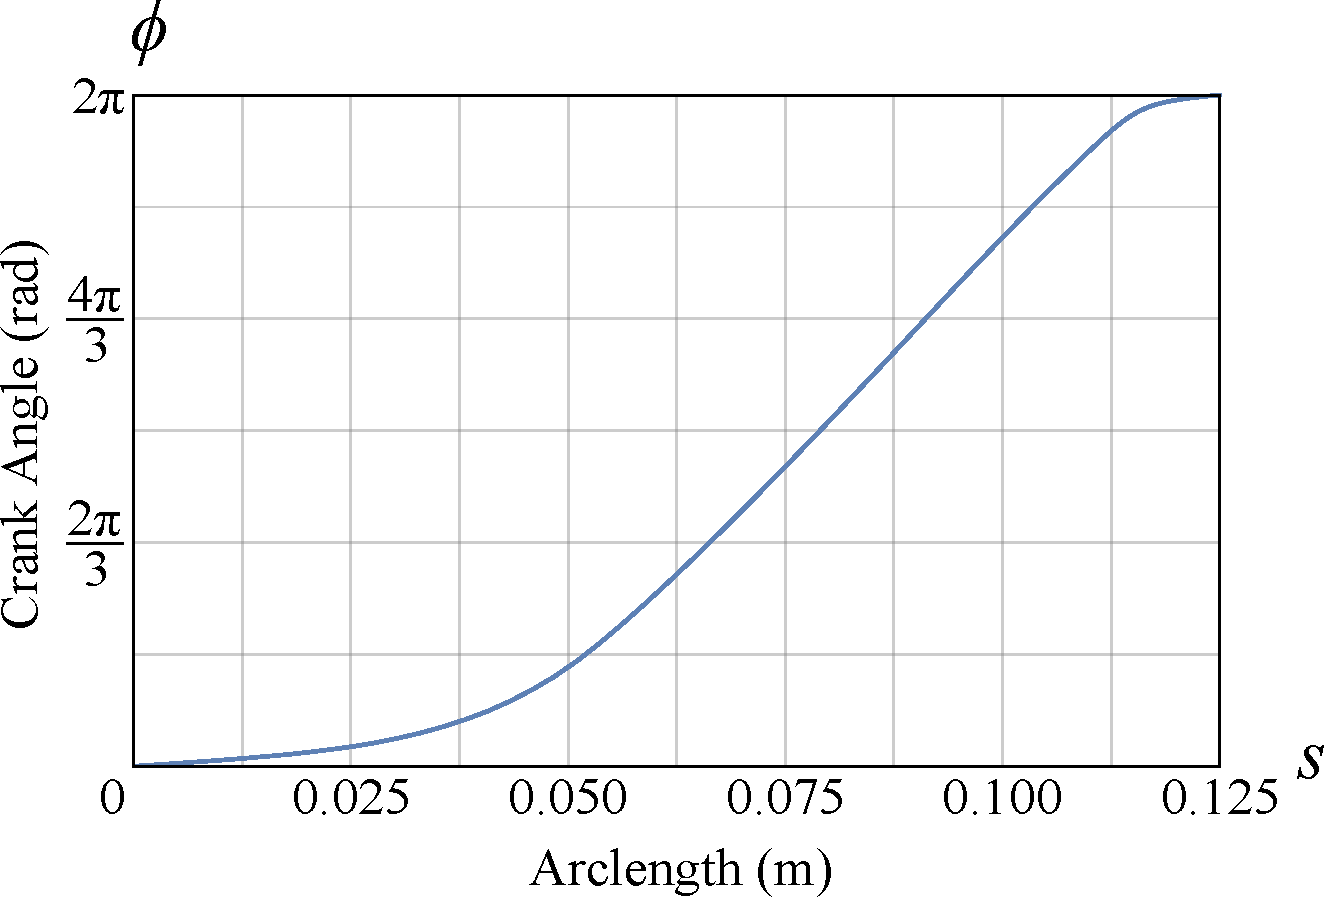
\includegraphics[scale=0.3]{clickspec_angle}%
\label{clickspec_angle}}
\caption{Mechanism properties were specified by clicking the red points on a computer screen and interpolating.  Specified properties are the \protect\subref{clickspec_path} the point trace path and \protect\subref{clickspec_ma} mechanical advantage coordinated with path arclength.  In \protect\subref{clickspec_angle}, the angle-arclength relationship is derived from integrating \protect\subref{clickspec_ma}.}
\label{clickspec}
\end{figure}

For example, the red points shown in Fig. \ref{clickspec_path} were clicked with a mouse.  The interpolated curve is parameterized by the Fourier series,
%\begin{equation}
%\begin{tabular}{cr}
%\multirow{3}[0]{*}{$\mathcal{C} = \begin{Bmatrix} \tilde{x}(t) \\ \tilde{y}(t) \end{Bmatrix}, \hspace{2mm} $}
%& $\tilde{x}(t) = \frac{1}{2}a_0 + \textstyle\sum\limits_{k=1}^{o}(a_k\cos 2\pi kt + b_k\sin 2\pi kt)$ \\
%& \vspace{-2mm} \\
%& $\tilde{y}(t) = \frac{1}{2}a_0 + \textstyle\sum\limits_{k=1}^{o}(a_k\cos kt + b_k\sin kt)$ \\
%\end{tabular}
%\end{equation}
\begin{align}
&\tilde{x}(\tau) = \tfrac{1}{2}a_0 + \textstyle\sum\limits_{k=1}^{o}\!\Big( a_k\cos (2\pi k\tau) + b_k\sin (2\pi k\tau) \Big) \nonumber\\[5pt]
&\tilde{y}(\tau) = \tfrac{1}{2}c_0 + \textstyle\sum\limits_{k=1}^{o}\!\Big( c_k\cos (2\pi k\tau) + d_k\sin (2\pi k\tau) \Big)
\label{fourier_interp_path}
\end{align}
%such that $\mathcal{C} = \{ (u,v) \;|\; u = \tilde{x}(t),\; v = \tilde{y}(t) \;\forall\; t \in [0,1] \}$
such that $\mathcal{C} = \left\lbrace \left( \tilde{x}(t), \tilde{y}(t) \right) |\; \tau \in [0,1] \right\rbrace$.
The values of Fourier coefficients for the example problem are displayed in Appendix \ref{app:fourier_coefficients}.
Order $o$ may be freely specified.


Next we replace parameter $\tau$ with arclength $s$.
To do this, we integrate along $\mathcal{C}$ to densely sample points $(s, \tau)$, then interpolate through them with a cubic Hermite spline creating a monotonic function for $\tau$ of $s$.  Substituting this function into Eqn. (\ref{fourier_interp_path}) yields a numerical arclength parameterization of $\mathcal{C}$,
\begin{align}
x(s) = \tilde{x}(\tau(s)), \nonumber\\
y(s) = \tilde{y}(\tau(s)).
\label{fourier_interp_path_arc}
\end{align}
Eqn. (\ref{fourier_interp_path_arc}) is valid for $s=[0,s_\text{total}]$, the arclength of the entire closed curve.

We follow a similar process for specifying mechanical advantage with a few modifications.
First, mechanical advantage $\gamma$ is defined as a function of normalized arclength $\hat{s}$ so that points are clicked with a mouse in the $\hat{s}$-$\gamma$ plane shown in Fig. \ref{clickspec_ma}.
Second, the endpoints at $\hat{s}\!=\!0$ and $\hat{s}\!=\!1$ are always specified and share the same $\gamma$ value.
And third, after interpolation the resulting Fourier series $\gamma(\hat{s})$ must be vertically shifted.
For a fully rotatable input crank, the area under $\gamma(\hat{s})$ must be $2\pi$.
To see this, note that mechanical advantage is equal to the ratio of input and output velocities,
\begin{equation}
\frac{d\phi}{d\hat{s}} = \gamma(\hat{s}).
\end{equation}
For a full traversal of $\mathcal{C}$, the crank must rotate $2\pi$, or rather
\begin{equation}
2\pi = \int_{0}^{1} \gamma(\hat{s}) d\hat{s}.
\end{equation}
Next, function $\gamma(\hat{s})$ is rewritten to accept a non-normalized arclength $s$ argument,
\begin{equation}
\gamma(s) := \frac{\gamma(s/s_\text{total})}{s_\text{total}}
\label{gamma_of_s}
\end{equation}
Note we take a notational liberty in Eqn. (\ref{gamma_of_s}) by redefining function $\gamma$ in terms of itself instead of making up new notation.
Integration of $\gamma(s)$ yields an angle-arclength relationship which creates the specified mechanical advantage,
\begin{equation}
\phi(s) = \int_{0}^{s_\text{total}} \gamma(s)ds + \text{constant}.
\end{equation}
For our example, this curve is plotted in Fig. \ref{clickspec_angle}.  For convenience, the constant of integration is chosen so that $\phi(0) = 0$.

\subsection{Equations of Motion}
\label{sec:eq_of_mot}

After specifying the characteristics of a to-be-designed linkage, Fig. \ref{clickspec}, the mock-up system illustrated in Fig. \ref{dynamic_model} may be simulated.

The motor dynamics obey a linear torque-speed law,
\begin{equation}
T = -\frac{T_\text{stall}}{\omega_\text{free}} \dot{\theta}_\text{m} + T_\text{stall},
\label{torque-speed}
\end{equation}
where $T_\text{stall}$ is stall torque and $\omega_\text{free}$ is free-running speed.

The torque transmitted through the spring follows
\begin{equation}
T = -k_\text{spring}(\phi - \theta_\text{m}) - c_\text{damp}(\dot{\phi} - \dot{\theta}_\text{m}),
\end{equation}
where $k_\text{spring}$ is stiffness and $c_\text{damp}$ is damping.

The mechanical advantage transformation from torque to output force is
\begin{equation}
F_t = T \gamma(s),
\end{equation}
where $F_t$ is the force acting on mass $m$ tangent to curve $\mathcal{C}$, and $\gamma(s)$ follows Eqn (\ref{gamma_of_s}).

\begin{figure}[!t]
\centering
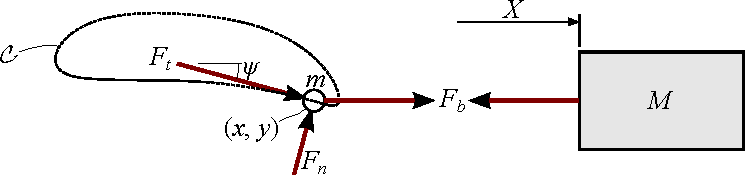
\includegraphics[scale=0.65]{dynamic_model_detail}
\caption{A detail of force notation at the interaction of $m$ and $M$.  Corresponds to Fig. \ref{dynamic_model}.}
\label{dynamic_model_detail}
\end{figure}

And finally, the forces acting on masses $m$ and $M$ follow the diagrams drawn in Fig. \ref{dynamic_model_detail}.
That is,
\begin{align}
&F_t\cos\nu - F_n\sin\nu - F_b = m\ddot{x}, \nonumber\\
&F_t\sin\nu + F_n\cos\nu = m\ddot{y}, \nonumber\\
&F_b = M\ddot{X},
\end{align}
and if $m$ and $M$ are in contact,
\begin{equation}
\ddot{x} = \ddot{X}
\end{equation}
else
\begin{equation}
F_b = 0.
\end{equation}
$F_n$ is the constraint force normal to $\mathcal{C}$, $F_b$ is the reaction force between $m$ and $M$, $(x,y)$ are the coordinates of $m$ constrained to $\mathcal{C}$ according to Eqn. (\ref{fourier_interp_path_arc}), $X$ is the coordinate of $M$, and $\psi$ is the tangency angle of $\mathcal{C}$ at $(x,y)$, that is
\begin{equation}
\nu = \arctan\frac{\dot{y}}{\dot{x}}.
\label{tangency_angle}
\end{equation}
Eqns. (\ref{torque-speed})--(\ref{tangency_angle}) in conjunction with $x(s)$, $y(s)$, $\gamma(s)$, and $\phi(s)$ specified in Section \ref{sec:spec_mech_char} form the equations of motion.  To solve these equations, they were rewritten into the form of an initial value problem for use with standard ODE solvers.



\subsection{Mock-Up Example}
\label{sec:mock_exam}

The mechanism characteristics shown in Fig. \ref{clickspec} were specified to create a recycling foot path with a fully rotatable crank that modulates the kinetic power of $M$ beyond the motor's limit along the bottom portion of $\mathcal{C}$.
These specifications were informed by intuition, past experience, and bio-inspiration \cite{haldaneRoboticVerticalJumping2016}.


\begin{figure}[!t]
\centering
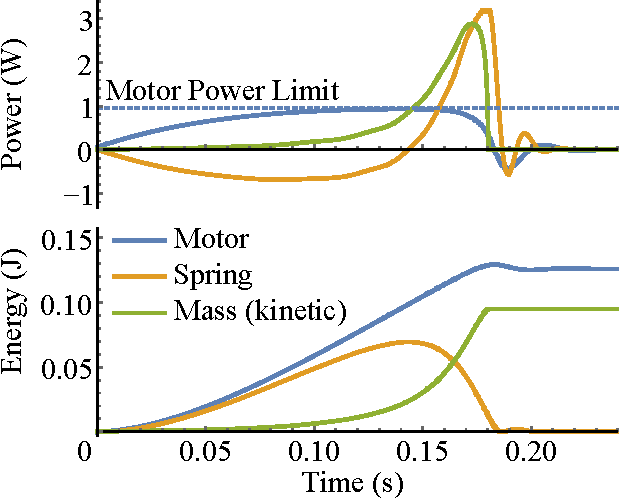
\includegraphics[scale=0.55]{simulation_results}
\caption{Simulation results of the model shown in Fig. \ref{dynamic_model} for the mechanism properties shown in Fig. \ref{clickspec}.  The mechanical power output associated with the mass surpasses the motor's limit.}
\label{simulation_results}
\end{figure}


\begin{table}[h]
\caption{Values of simulation parametes}
\label{simulation_parameters}
\centering
\begin{tabular}{|m{6mm}|r@{ }l|m{48mm}|}
\hline
\textbf{Para-meter} & \multicolumn{2}{c|}{\textbf{Value}} & \textbf{Comment} \\
\hline
$T_\text{stall}$ & 0.33 & Nm & \multirow{2}[4]{*}{Pololu 298:1 Micro Metal Gearmotor} \\
\cline{1-3}$\omega_\text{free}$ & 11.5 & rad/s &  \\
\hline
$k_\text{spring}$ & 0.14 & Nm/rad & 14 mm cylindrical cut of latex \\
\hline
$c_\text{damp}$ & 0.0005 & Nm/(rad/s) & Estimated \\
\hline
$m$ & 0.02 & kg & Stand-in for to-be-designed linkage inertia \\
\hline
$M$ & 0.23 & kg & Typical mass of small robot \\
\hline
\end{tabular}
\end{table}


The values of physical parameters are displayed in Table \ref{simulation_parameters}.
The results of numerical simulation are shown in Fig. \ref{simulation_results}.
Simulation shows that modulation of motor power by a factor of 3.0 is possible.
A leg designed with these mechanical characteristics might deliver 95 mJ of kinetic energy in one stance phase.


\section{Synthesis Equations}
\label{sec:synth_eq}

After determining desired mechanism characteristics in Section \ref{sec:dynamic_mock-up}, our objective is to synthesize a linkage that exhibits those characteristics.
In particular, we desire a physical instantiation of $x(s)$, $y(s)$, and $\phi(s)$.
The latter of the three is desired more so for its derivative, $\gamma(s)$, rather than itself, but we employ it directly as a design goal nonetheless.
The design problem of finding a linkage that creates a desired endpoint path is called \emph{path generation}.
When this path is additionally coordinated with the angle of an input crank, this problem is sometimes called \emph{timed curve generation} \cite{dijksmanMotionGeometryMechanisms1976}.


In this section, we solve this problem for a Stephenson II six-bar.  The choice to investigate six-bars is not arbitrary.  These linkages are capable of single degree-of-freedom motions which are much more complex than four-bars, the next simplest single degree-of-freedom linkage.  However, the choice to particularly investigate the Stephenson II type of six-bar is partially arbitrary.  There are other types worth investigation too which are not considered in this work.  Before this paper, complete solutions for any type of six-bar timed path generator have not been computed.


Specifically, we formulate the synthesis equations for a Stephenson II six-bar linkage to track an endpoint attached to one of its floating binary links through eight positions that are coordinated with its binary input crank angle.
Later in Section \ref{sec:frg}, these equations are solved for the first time.


\subsection{Formulation}
\label{sec:synth_form}

\medmuskip=2mu
A Stephenson II six-bar linkage is drawn in Fig. \ref{synthesis_diagram}.  It is composed of seven joints.  Fig. \ref{synthesis_diagram} displays a reference configuration and the $j^\text{th}$ displaced configuration.  There are $N-1$ displaced configurations.  Joint coordinates in the reference configuration are stored in the real and imaginary components of the complex numbers $A$, $B$, $C$, $D$, $F$, $G$, and $H$.  The coordinates of the end effector point in the reference configuration is $P_0$ and in the $j^\text{th}$ displaced configuration is $P_j$.  The angular displacement of each of the five moving links is measured by $\phi_j$, $\rho_j$, $\psi_j$, $\theta_j$, and $\mu_j$ as marked in Fig. \ref{synthesis_diagram}.
\medmuskip=4mu

\begin{figure}[!t]
\centering
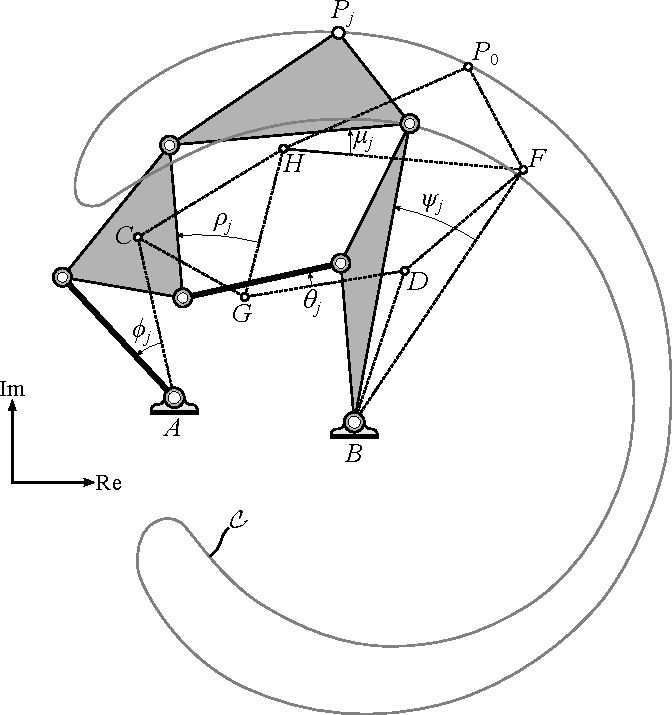
\includegraphics[width=1\linewidth]{synthesis_diagram}
\caption{Diagram describing the notation used in the synthesis formulation.  Linkage pivots in a reference configuration are marked with complex numbers $A$, $B$, $C$, $D$, $F$, $G$, and $H$.  The $j^\text{th}$ displaced configuration is shown here.}
\label{synthesis_diagram}
\end{figure}



Planar vectors written in complex form may be rotated by multiplication with rotation operators,
\begin{align}
&Q_j = e^{i\phi_j}, \quad R_j = e^{i\rho_j}, \quad S_j = e^{i\psi_j}, \nonumber\\
&\hspace{8mm} T_j = e^{i\theta_j}, \quad U_j = e^{i\mu_j}, \qquad j=1,\ldots,N-1.
\end{align}

\medmuskip=2mu
For our synthesis problem of interest, we take it that all values of crank rotation $Q_j$, $j=1,\ldots,N-1$ and end point position $P_j$, $j=0,\ldots,N-1$ are known.  All other symbols are variables to be solved for or eliminated.  Note the index $j=0$ does not exist for $Q_j$ because this simply refers to the reference configuration.
\medmuskip=4mu

To begin deriving the synthesis equations, first form three independent vector loop equations from Fig. \ref{clickspec},
\medmuskip=2mu
\begin{align}
&R_j(H-C) = P_j - A - Q_j(C-A) - U_j(P_0-H) \label{loopR1}\\
&S_j(F-B) = P_j - B - U_j(P_0-F) \label{loopS1}\\
&T_j(G-D) = A-B + Q_j(C-A) + R_j(G-C) - S_j(D-B) \label{loopT1}\\
&\hspace{50mm} j=1,\ldots,N-1 \nonumber
\end{align}
\medmuskip=4mu

To eliminate $R_j$, $S_j$, and $T_j$ from these equations.
Eqns. (\ref{loopR1}) and (\ref{loopS1}) are solved for $R_j$ and $S_j$, respectively, then substituted into (\ref{loopT1}).  The result is then multiplied by its own conjugate.  Eqns. (\ref{loopR1}) and (\ref{loopS1}) are also multiplied by their own conjugates.  After partial expansion, this yields the equations below.  The overbar denotes conjugation.
%\medmuskip=4mu
%\begin{align}
%U_j(P_0-H)\big(\*P_j-\*A-\*Q_j(\*C-\*A)\big) \nonumber\\
%+ U_j(P_0-H)\big(\*P_j-\*A-\*Q_j(\*C-\*A)\big) \nonumber\\
%+ Q_j(C-A)(\*P_j-\*A) + Q_j(C-A)(\*P_j-\*A) \nonumber\\
%+ A(\*P_j+\*C-\*A) + A(\*P_j+\*C-\*A) \nonumber\\
%+ H(\*P_0-\*C) + H(\*P_0-\*C) - P_j\*P_j - P_0\*P_0 = 0 \\
%%
%U_j(P_0-F)(\*P_j-\*B) + U_j(P_0-F)(\*P_j-\*B) + P_j\*B + P_j\*B \nonumber\\
%+ F(\*P_0-\*B) + F(\*P_0-\*B) - P_j\*P_j - P_0\*P_0 = 0 \\
%%
%U_j\bigg(\frac{G-C}{H-C}(P_0-H)-\frac{D-B}{F-B}(P_0-F)\bigg) \nonumber\\
%\times \bigg(\*A-\*B+\*Q_j(\*C-\*A) + \frac{\*G-\*C}{\*H-\*C}\big(\*P_j-\*A-\*Q_j(\*C-\*A)\big) \nonumber\\
% - \frac{\*D-\*B}{\*F-\*B}(\*P_j-\*B)\bigg) \nonumber\\
%- \bigg(A-B+Q_j(C-A)+\frac{G-C}{H-C}\big(P_j-A-Q_j(C-A)\big) \nonumber\\
%-\frac{D-B}{F-B}(P_j-B)\bigg)
%\end{align}
%\medmuskip=4mu
%where the overbar notation denotes the conjugate.
\begin{align}
&\beta_j + \*\beta_j - P_j\*P_j - P_0\*P_0 = 0 \label{loopbeta1}\\
&\xi_j + \*\xi_j - P_j\*P_j - P_0\*P_0 = 0 \label{loopxi1}\\
&U_j\lambda\*\zeta_j + \*U_j\*\lambda\zeta_j - \zeta_j\*\zeta_j - \lambda\*\lambda + (G\!-\!D)(\*G\!-\!\*D) = 0 \label{loopzeta1} \\
&\hspace{50mm} j=1,\ldots,N-1 \nonumber
\end{align}
The new intermediate variables $\beta_j$, $\xi_j$, $\zeta_j$, $\lambda$ are introduced only for compact presentation and illustrating equation structure.  They are defined
\medmuskip=2mu
\begin{align}
&\beta_j = U_j(P_0-H)\big(\*P_j-\*A-\*Q_j(\*C-\*A)\big) + \nonumber\\
&\hspace{10mm} Q_j(C-A)(\*P_j-\*A) + A(\*P_j+\*C-\*A) + H(\*P_0-\*C), \nonumber\\
&\xi = U_j(P_0-F)(\*P_j-\*B) + P_j\*B + F(\*P_0-\*B), \nonumber\\
&\zeta_j = A-B+Q_j(C-A) + \nonumber\\
&\hspace{10mm} \frac{G-C}{H-C}\big(P_j-A-Q_j(C-A)\big) - \frac{D-B}{F-B}(P_j-B), \nonumber\\
&\lambda = \frac{G-C}{H-C}(P_0-H)-\frac{D-B}{F-B}(P_0-F). \label{expansion1}
\end{align}
\medmuskip=4mu
Conjugates $\*\beta_j$, $\*\xi_j$, $\*\zeta_j$, $\*\lambda$ are defined as expected.  Eqns. (\ref{loopbeta1})--(\ref{loopzeta1}) were simplified by the fact that a rotation operator multiplied by its conjugate equals one, eliminating $R_j$, $S_j$, and $T_j$.  The remaining unknown rotation operator is $U_j$.  Its values must obey
\begin{equation}
U_j \*U_j = 1.
\label{Unorm}
\end{equation}



In order to estimate the number of roots of our synthesis system, we convert Eqns. (\ref{loopbeta1})--(\ref{loopzeta1}) to polynomials.
To do this, we first change our interpretation of the overbar.  Rather than a conjugate operation, variables with an overbar are considered separate unknowns.  
That is, instead of considering the coordinated pair $\big(\operatorname{Re}[A], \, \operatorname{Im}[A]\:\big)$, we consider isotropic coordinates $(A, \*A\:)$ \cite{wamplerIsotropicCoordinatesCircularity1996}.  The two are separated by an invertible linear transformation,
\begin{equation}
\begin{Bmatrix} A \\ \*A \end{Bmatrix} =
\begin{bmatrix} 1 & i \\ 1 & -i \end{bmatrix}
\begin{Bmatrix} \operatorname{Re}[A] \\ \operatorname{Im}[A] \end{Bmatrix}
\end{equation}
Next, we introduce the following substitutions to make Eqn. (\ref{loopzeta1}) polynomial and help reduce the total degree of our synthesis system,
\medmuskip=0mu
\begin{align}
a &= A\*H, & \*a &= \*AH, \label{sub1}\\
b &= B\*F, & \*b &= \*BF, \label{sub2}\\
c &= (C-A)\*H, & \*c &= (\*C-\*A)H, \label{sub3}\\
d &= \frac{D-B}{F-B}, & \*d &= \frac{\*D-\*B}{\*F-\*B}, \label{sub4}\\
g &= \frac{G-C}{H-C}, & \*g &= \frac{\*G-\*C}{\*H-\*C}, \label{sub5}\\
k &= g(P_0-H) - d(P_0-F), & \*k &= \*g(\*P_0-\*H) - \*d(\*P_0-\*F). \label{sub6}
\end{align}
\medmuskip=4mu

Substituting Eqns. (\ref{sub1})--(\ref{sub6}) into Eqns. (\ref{loopbeta1})--(\ref{loopzeta1}) obtains
\begin{align}
&\beta_j + \*\beta_j - P_j\*P_j - P_0\*P_0 = 0 \\
&\xi_j + \*\xi_j - P_j\*P_j - P_0\*P_0 = 0 \\
&U_jk\*\zeta_j + \*U_j\*k\zeta_j - \zeta_j\*\zeta_j - k\*k \; + \nonumber\\ 
&\hspace{10mm} \Big(g(H\!-\!C)\!+\!C\!-\!d(F\!-\!B)\!-\!B\Big) \times \nonumber\\
&\hspace{10mm} \Big(\*g(\*H\!-\!\*C)\!+\!\*C\!-\!\*d(\*F\!-\!\*B)\!-\!\*B\Big) = 0 \\
&\hspace{50mm} j=1,\ldots,N-1 \nonumber
\end{align}
where
\medmuskip=2mu
\begin{align}
&\beta_j = U_j \Big(P_0 \big(\*P_j-\*A-\*Q_j(\*C-\*A)\big) - \*P_jH+\*a+\*Q_j\*c\Big) + \nonumber\\
&\hspace{10mm} Q_j(C-A)(\*P_j-\*A) + A(\*P_j+\*C-\*A) + H(\*P_0-\*C), \nonumber\\
&\xi_j = U_j \big(P_0(\*P_j-\*B) - \*P_jF + \*b\big) + P_j\*B + P_0\*F - b, \nonumber\\
&\zeta_j = A-B+Q_j(C-A) + \nonumber\\
&\hspace{20mm} g\big(P_j-A-Q_j(C-A)\big) - d(P_j-B). \label{loopzeta2}
\end{align}
\medmuskip=4mu
When $N=8$, Eqns. (\ref{sub1})--(\ref{sub3}), (\ref{sub6})--(\ref{loopzeta2}) are 36 equations in 36 unknowns:
\begin{align}
&\left\lbrace A, \*A, B, \*B, C, \*C, F, \*F, H, \*H, a, \*a, b, \*b, c, \*c, d, \*d, g, \*g, k, \*k \right\rbrace, \nonumber\\
&\left\lbrace U_j, \*U_j \right\rbrace, \qquad j=1,\ldots,7.
\end{align}
The total degree of this system is $2^7 2^8 2^7 2^7 4^7$ $\approx$ $8.8\!\times\!10^{12}$, which is an overestimated ceiling on the maximum number of finite roots.  After applying FRG in the next section, we estimate the true number to be near $1.5\!\times\!10^{6}$.


\section{Finite Root Generation}
\label{sec:frg}


Finite Root Generation (FRG) was first proposed in \cite{plecnikFindingOnlyFinite2017}.
The method is based in homotopy continuation and is used for solving kinematic synthesis systems with large numbers of roots.

Generally, homotopy solvers work to find all the roots of a polynomial \emph{target system} by first constructing a polynomial \emph{start system} with easily obtainable roots and a monomial structure at least more general than that of the target system.
Then, a homotopy between the systems is constructed and start system roots, \emph{startpoints}, are tracked continuously to target system roots, \emph{endpoints}.
Through this method all finite roots of the target system will be found.

Start systems are commonly constructed as products of linear expressions in order to easily obtain all their roots.
By picking one linear expression from each equation, then solving the resulting square linear system, a startpoint is found.  
Doing this for all valid combinations of linear expressions finds all startpoints.
The problem arises that a start system constructed this way tends to comprise of many more monomials than the target system, which tends to have a sparse structure for the problems of interest.
This usually means there will be drastically more finite startpoints than endpoints, with the far majority of homotopy paths tracking toward roots at infinity.


FRG solves this problem by constructing start systems with the exact monomial structure as the target system.
This is accomplished by generating a random linkage and extracting a start system from its motion and a startpoint from its dimensions.
This single startpoint will indeed track to a finite root of the target system.
To get a second root, this process is repeated.
As the finite target root set we aim to obtain is very large, chances are that this second startpoint will track to a different endpoint, with no guarantee.
Repeating this process, roots are accumulated.
As FRG trials progress, eventually the odds of acquiring a new root become unfavorable.
More and more duplicate roots are computed.
FRG trades away infinite root computations for duplicate root computations.  
For sparse systems, the latter tends to be far fewer than the former, making it a good trade.
The frequency of duplicate roots was characterized in \cite{plecnikStudyFindingFinite2017}.
Tracking their occurrence allows an in-process estimate of the percentage of the total root set that has been obtained.

FRG mediates additional computation savings by exploiting known solution structures in a straightforward way.
For linkage synthesis equations, this structure is primarily provided by the presence of linkage cognates.
The cognate of a single degree-of-freedom linkage is another linkage with different dimensions that exactly reproduces some aspect of the original linkage's continuous motion.
For a given linkage type (e.g. Stephenson II) and motion of interest (e.g. timed curve generation), the presence and number of cognates is often known.
As well, geometric transformations between cognates are known too.
Using these transformations, an entire set of cognate roots can be quickly computed from one endpoint.
Each root in a cognate set is a separate isolated solution, and cognate sets have no intersection with each other.
Combining cognate structures with other existing symmetries (if present) partitions target roots into a smaller number of sets, thereby reducing the expected computational load by the multiple of the size of a single solution set.


Finally, any time one intends to solve several systems within a specific family, this is accomplished efficiently using the parameter homotopy method.
That is, in order to solve a new instance of our synthesis system, say for a different set of task parameters, we do not need to start from scratch.
First, all roots are found for a numerically general member of the family of systems of interest.
This is called an \emph{ab initio} solution and may be found using any method, in our case FRG.
The ab initio roots may then serve as startpoints for a homotopy that transforms parameters of the ab initio system into any other member of the family of interest.
These subsequent parameter homotopies only need to track as many paths as the number of roots from the ab initio system, saving computational effort.
Following this strategy, the synthesis system solved below is for ab initio task parameters specified as random complex numbers that do not correspond to anything physical.
In Section \ref{sec:leg_app}, this ab initio solution is used as the start in parameter homotopies for physical relevant target systems.









\subsection{Reformulation of Synthesis Equations}
\label{sec:reform_synth_eq}

Unlike other homotopy-based solvers, FRG does not compute roots from a start system generated to match a B\'{e}zout number calculation.
Therefore, rather than moving forward with the formulation of our synthesis system presented in Eqns. (\ref{sub1})--(\ref{sub3}), (\ref{sub6})--(\ref{loopzeta2}), we choose a formulation with fewer equations and unknowns, Eqns. (\ref{loopbeta1})--(\ref{Unorm}).
This formulation is further reduced by substituting $\*U_j = 1/U_j$, $j=1,\ldots,7$ into Eqns. (\ref{loopbeta1})--(\ref{loopzeta1}) to eliminate 7 more variables. 
Although these equations are not polynomial, FRG applies without modification.
We name this system $\mathcal{S}$, its variables $\mathbf{z}$, and its defining parameters $\mathbf{q}$,
\begin{equation}
\mathcal{S}(\mathbf{z},\mathbf{q}) = 0.
\label{system}
\end{equation}
The vector of variables $\mathbf{z}$ contains the unknowns we intend to solve for
\begin{align}
\mathbf{z} = \{ \mathbf{A}, &\mathbf{U} \}, \label{z_variables}\\
\text{where} \quad
\mathbf{A} &= \{ A, B, C, D, F, G, H, \*A, \*B, \*C, \*D, \*F, \*G, \*H \}, \nonumber\\
\mathbf{U} &= \{ U_1, \ldots, U_7 \}. \nonumber
\end{align}
The vector of parameters $\mathbf{q}$ defines the system we are attempting to solve
\begin{align}
\mathbf{q} = \{\mathbf{P}, \*{\mathbf{P}}, &\mathbf{Q}, \*{\mathbf{Q}} \} & & \label{q_parameters}\\
\text{where} \quad
\mathbf{P} &= \{ P_0, \ldots, P_7 \}, & \*{\mathbf{P}} &= \{ \*P_0, \ldots, \*P_7 \}, \nonumber\\
\mathbf{Q} &= \{ Q_1, \ldots, Q_7 \}, & \*{\mathbf{Q}} &= \{ \*Q_1, \ldots, \*Q_7 \}. \nonumber
\end{align}



\subsection{Constructing Start Systems}
\label{sec:start_sys}


Each FRG iteration begins with the generation of a single startpoint and corresponding start system.  A startpoint is defined by a vector of variables $\mathbf{z}$ (Eqn. (\ref{z_variables})) and a start system is defined by a vector of parameters $\mathbf{q}$ (Eqn. (\ref{q_parameters})).
To generate a pair $(\mathbf{z}, \mathbf{q})$ that satisfies Eqn. (\ref{system}), some values are randomly generated and others are computed from those values.
First, random complex values are assigned to $\mathbf{A}$, $P_0$, and $\*P_0$.  
Values were chosen from a square in the complex plane with corners $-5-5i$ and $5+5i$.
Variables with the overbar notation were not chosen to be conjugate to their non-overbar counterparts, but were also randomly selected, abandoning their physical meaning.

Although physically relevant values were not used, the rest of the variables and parameters within $\mathbf{z}$ and $\mathbf{q}$ are computed from the forward kinematics equations of a physical six-bar model.
Physical or not, the result still satisfies Eqn. (\ref{system}), which is our goal at the moment.
These forward kinematics equations are included in Appendix \ref{app:fwd_kin}.
As a six-bar is a one degree-of-freedom linkage, in order to extract random configurations from its motion, we must provide random values for a single configuration parameter.
We choose $R_j\*U_j$, $j=1,\ldots,7$, the complex number associated with angle $\rho_j-\mu_j$, because it makes the forward kinematics computations simple and fast.
It may be noted that the complexity of the solution process of the forward kinematics is dependent on the choice of a specified configuration parameter.
Perhaps intuitively, $R\*U$ is a good choice because it defines one angle of the floating four-bar $DGHF$, which segments calculations to one variable at a time after that.
Solving the forward kinematics equations provides all remaining values in $\mathbf{z}$ and $\mathbf{q}$.
A homotopy path may then be tracked from the startpoint $\mathbf{z}$ that solves the system defined by $\mathbf{q}$ to a finite root that solves our target system, Eqn. (\ref{system}).




\subsection{Cognate Structure}
\label{sec:cognates}

The roots of $\mathcal{S}$ are organized into the structure afforded by the linkage cognates of a Stephenson II timed curve generator.
More specifically, we are dealing with a Stephenson II where the trace point is connected to one of the floating binary links.
We also could have attached the trace point to ternary link $CGH$.
In this case, the mechanism would still be useful but the results here do not apply.

Dijksman has enumerated the timed curve cognates we seek \cite[pg.~183]{dijksmanMotionGeometryMechanisms1976}.  There are four.
Their geometric construction is outlined in \cite{dijksmanSixBarCognatesStephenson1971}.
Here we present their equations.


Given a linkage defined by $\mathbf{X}$,
\begin{equation}
\mathbf{X} = \{ A, B, C, D, F, G, H, P_0 \},
\end{equation}
its first two cognates are called the 1/2-cognate and 3/4-cognate.

To obtain the 1/2 cognate, we define a map $\kappa_{1/2} : \mathbb{C}^8 \mapsto \mathbb{C}^8$,
\begin{align}
&\hspace{-10mm}
\kappa_{1/2}(\mathbf{X}) := 
\begin{Bmatrix}
(\Lambda\circ\Gamma)(A) \\
B \\
(\Lambda\circ\Gamma)(C) \\
\Lambda(D) \\
F \\
(\Lambda\circ\Gamma)(G) \\
\Lambda(H) \\
P_0
\end{Bmatrix} \label{cognates12}\\[2mm]
\text{where} \quad
&\Gamma(z) := \dfrac{H-G}{C-G}(z-D)+D \nonumber\\
&\Lambda(z) := \dfrac{B-F}{\Gamma(B)-F}(z-F)+F \nonumber
\end{align}


To obtain the 3/4 cognate, we define a map $\kappa_{3/4} : \mathbb{C}^8 \mapsto \mathbb{C}^8$,
\begin{align}
&\hspace{-10mm}
\kappa_{3/4}(\mathbf{X}) := 
\begin{Bmatrix}
\Upsilon(A) \\
B \\
\Upsilon(C) \\
(\Upsilon\circ\Xi)(D) \\
B+P_0-F \\
(\Upsilon\circ\Xi)(G) \\
\Upsilon(H) \\
P_0
\end{Bmatrix} \label{cognates34}\\[2mm]
\text{where} \quad
&\Xi(z) := \dfrac{B-F}{D-F}(z-H)+H \nonumber\\
&\Upsilon(z) := \dfrac{P_0-F}{H-F}(z-B)+B \nonumber
\end{align}

\medmuskip=1mu
To gain some geometric intuition on $\Gamma$, $\Lambda$, $\Xi$, and $\Upsilon$, note that they take the form of a stretch-rotation about a pole.  
For example, $\Gamma$ may be interpreted as a rotation of $\angle HGC$\footnote{To be more precise, this is the angle that rotates $\overline{GH}$ to lie parallel with $\overline{GC}$ (not vice versa).  The ``$\angle$'' notation does not convey direction.} about $D$ combined with a dilation by $|H-G|/|C-G|$ centered on $D$.  Both $\kappa_{1/2}$ and $\kappa_{3/4}$ are their own inverses,
\medmuskip=4mu
\begin{equation}
\kappa_{1/2}^{-1} \equiv \kappa_{1/2}, \qquad \kappa_{3/4}^{-1} \equiv \kappa_{3/4}.
\end{equation}

The final cognate is called the 1/2-3/4 cognate.  It is obtained from the commutative composition of $\kappa_{1/2}$ and $\kappa_{3/4}$,
\begin{equation}
\kappa_{1/2\text{-}3/4} := \kappa_{1/2} \circ \kappa_{3/4} \equiv \kappa_{3/4} \circ \kappa_{1/2}. \label{cognates1234}
\end{equation}


Following Eqns. (\ref{cognates12}), (\ref{cognates34}), and (\ref{cognates1234}), the set of six-bars defined by 
\begin{equation}
%\mathsf{C} = 
\left\lbrace
\mathbf{X}, \;
\kappa_{1/2}(\mathbf{X}), \;
\kappa_{3/4}(\mathbf{X}), \;
(\kappa_{1/2}\circ\kappa_{3/4})(\mathbf{X})
\right\rbrace
\end{equation}
all trace the exact same coupler curve with the exact same angular displacement of crank $AC$.

These equations demonstrate how to transform a linkage into its cognates.
To be useful for FRG, we need to transform a solution $\mathbf{z}$ of the form shown in Eqn. (\ref{z_variables}) to its cognate solutions.

For the 1/2-cognate solution, we need only to append conjugate unknowns and duplicate the vector $\mathbf{U}$ (Eqn. (\ref{z_variables})),
\begin{equation}
\mathbf{z}_{1/2} = \Big\{
\kappa_{1/2}(\mathbf{X}), \;
\kappa_{1/2}(\*{\mathbf{X}}), \;
\mathbf{U} \Big\}.
\label{soln_cogns_12}
\end{equation}

For the 3/4- and 1/2-3/4 cognate solutions, we append conjugate unknowns and transform the vector $\mathbf{U}$ according to the geometric construction given in \cite{dijksmanSixBarCognatesStephenson1971},
\begin{align}
\mathbf{z}_{3/4} &= \Big\{
\kappa_{3/4}(\mathbf{X}), \;
\kappa_{3/4}(\*{\mathbf{X}}), \;
\mathbf{U}' \Big\} \label{soln_cogns_34_1234}\\
%
\mathbf{z}_{1/2\text{-}3/4} &= \Big\{
(\kappa_{1/2}\circ\kappa_{3/4})(\mathbf{X}), \;
(\kappa_{1/2}\circ\kappa_{3/4})(\*{\mathbf{X}}), \;
\mathbf{U}' \Big\} \nonumber\\[2mm]
%
\text{where} 
&\hspace{5mm} \mathbf{U}' = \{ U'_1, \ldots, U'_7 \}, \nonumber\\
&\hspace{5mm}  U'_j = \dfrac{P_j-B-U_j(P_0-F)}{F-B} \quad j=1,\ldots,7. \nonumber
\end{align}

Unfortunately, Eqns. (\ref{soln_cogns_34_1234}) only apply to cases where corresponding components $Q_j$ and $\*Q_j$ of $\mathbf{q}$ (Eqn. (\ref{q_parameters})) are defined to be reciprocal.
The start systems constructed in Section \ref{sec:start_sys} and the target system constructed for the ab initio solve were defined with $Q_j$ and $\*Q_j$, $j=1,\ldots,7$ as unrelated random complex numbers.
Therefore, only Eqn. (\ref{soln_cogns_12}) applies to them, reducing the size of our cognate sets to two.
Defining $Q_j$ and $\*Q_j$ as reciprocal for start systems was possible, but this increased the numerical precision needed for path tracking such that the cost outweighed the benefit.
With cognate sets of size two, the expected amount of computation is cut in half.
For every finite root found, its cognate partner is readily computed from Eqn. (\ref{soln_cogns_12}).
To find all roots, we only must find all cognate sets, of which there are half as many.


\subsection{Computational Work}
\label{sec:computations}

Using the start system construction method of Section \ref{sec:start_sys} and exploiting the cognate structure of Section \ref{sec:cognates}, FRG was applied to find the ab initio roots $\mathbf{z}$ of a numerically general target system $\mathcal{S}(\mathbf{z},\mathbf{q}_1)=0$.
Target parameters $\mathbf{q}_1$ were randomly generated and are printed in Appendix \ref{app:fpm}.
After generating this ab initio solution, these roots were used repeatedly in conjunction  with the parameter homotopy method to solve for any other system $\mathcal{S}(\mathbf{z},\mathbf{q}_2)=0$, where $\mathbf{q}_2$ might be defined by a specific synthesis task.
In Section \ref{sec:leg_app}, we will define $\mathbf{q}_2$ according to analyses in Section \ref{sec:dynamic_mock-up}, to design a novel machine.



A single FRG iteration consists of generating a random startpoint/start system (Section \ref{sec:start_sys}), tracking a homotopy path from this startpoint to an endpoint root of the target system, computing the cognate set of that endpoint (Section \ref{sec:cognates}), and finally checking whether the cognate set found is a duplicate from a previous iteration.
By tracking the occurrence of duplicates, and assuming equal probability of happening upon any root of the target set during each iteration, an in-process estimate of the number of finite roots found is computed.
The algorithm ends when this estimate is sufficiently high.

Tracking a homotopy path involves following the values of root $\mathbf{z}$ from its startpoint $\mathbf{z} = \mathbf{z}_0$ that solves the start system $\mathcal{S}(\mathbf{z},\mathbf{q}_0)=0$, to its endpoint $\mathbf{z} = \mathbf{z}_1$ that solves the target system $\mathcal{S}(\mathbf{z},\mathbf{q}_1)=0$.
Path tracking was performed using a predictor-corrector technique based on Runge-Kutta and Newton iterations.  
This technique is presented in Appendix \ref{app:tracking}.


\begin{figure}[!t]
\centering
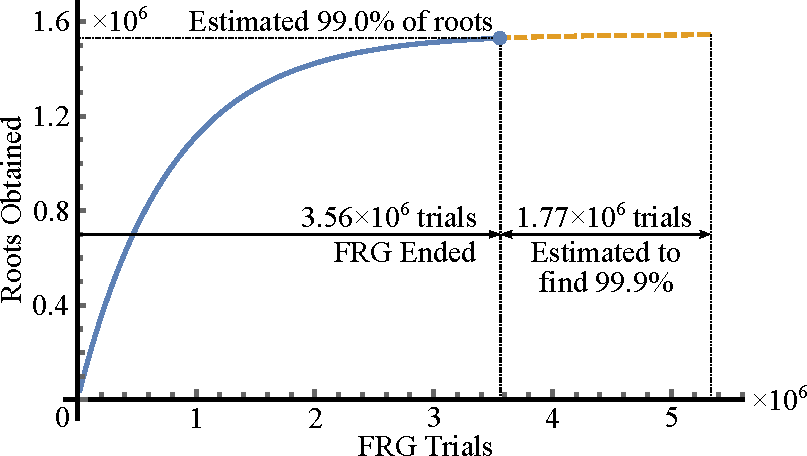
\includegraphics[scale=0.6]{frg_results}
\caption{The accumulation of roots over the procession of the FRG algorithgm.  An estimated 99.0\% of roots were found in $3.56 \times 10^6$ trials.  To find 99.9\% would take about 50\% more computational effort.}
\label{frg_results}
\end{figure}


FRG was written in CUDA and run on a laptop GPU for 3,563,520 trials over 24 hours.
It found 764,894 distinct cognate sets indicating 1,529,788 finite roots.
Of these, 1180 roots were suspected of being singular due to high condition numbers and so were discarded, leaving 1,528,608 isolated solutions.
According to the FRG estimation technique, this is 99.0\% of roots.  About 0.14\% of paths ended in numerical failure, usually from the Newton corrector step not converging due to precision limitations.  Fig. \ref{frg_results} displays root accumulation over FRG iterations.  The diminishing returns of FRG is documented in \cite{plecnikStudyFindingFinite2017}.  We estimate the algorithm would have found 99.9\% of roots with $1.77\times 10^6$ more trials.



\section{Application to Leg Mechanism}
\label{sec:leg_app}

The ab initio implementation of FRG presented in Section~\ref{sec:computations} found nearly all finite roots for a numerically general system $\mathcal{S}(\mathbf{z},\mathbf{q}_1)=0$.
This root set can be used to efficiently solve systems of the form $\mathcal{S}$ henceforth.
Parameter homotopies can be constructed that use these roots as startpoints to track to the roots of some other systems of the form $\mathcal{S}(\mathbf{z},\mathbf{q}_2)=0$.
However, the vector of parameters $\mathbf{q}$ (defined in Eqn. (\ref{q_parameters})) for these systems were composed of physical specifications informed by the analysis of Section \ref{sec:dynamic_mock-up}.

When physically relevant values of $\mathbf{q}$ are specified, some of the roots $\mathbf{z}$ (defined in Eqn. (\ref{z_variables})) of system $\mathcal{S}$ will be physically relevant as well.
These roots contain the pivot locations (design parameters) of six-bar linkages that produce the kinematic characteristics encoded in $\mathbf{q}$.
These kinematic characteristics were chosen to instantiate some dynamic behavior as informed by simplified simulations (Section \ref{sec:dynamic_mock-up}).
Bringing this all together forms a design process capable of finding six-bar linkages that produce some dynamic behavior under known loading conditions.
In this way, the ab initio root set obtained in Section \ref{sec:computations} serves as an instrument for designing dynamic machines.



To demonstrate this process, we design a leg mechanism for a small running robot capable of producing propulsive motions with energetics beyond its motor's power output.
We continue from the task specification introduced in Section \ref{sec:dynamic_mock-up}, where we established a cyclic path and coordinated crank angle function that would dynamically modulate the power output of a series-elastic actuator under load to increase kinetic energy during push-off of a single stance phase.
This task was transferred to a vector $\mathbf{q}_\text{task}$ by picking eight end effector positions $(x_j,y_j)$ and coordinated crank angles $\phi_j$, printed in Table \ref{task_parameters}.  Components of $\mathbf{q}_\text{task}$ are specified as
\begin{align}
P_j &= x_j + iy_j, & \*P_j &= x_j - iy_j, & j&=0,\ldots,7 \nonumber\\
Q_j &= e^{i\phi_j}, & \*Q_j &= e^{-i\phi_j}, & j&=1,\ldots,7 
\end{align}
Note that $(Q_0,\*Q_0)$ is automatically specified as $(1,1)$ without loss of generality, making the number of angles eight.

\begin{table}[h]
\caption{Specification of $\mathbf{q}_\text{task}$ for the leg mechanism example.}
\label{task_parameters}
\centering
\begin{tabular}{c|r@{}lc}
$j$ & \multicolumn{2}{c}{$P_j$ (cm)} & \multicolumn{1}{c}{$\phi_j$ (rad)} \\
\hline
0 & 0.09504886 & $+$0.06372449$i$ & 0 \\
1 & 0.90856802 & $-$0.19472945$i$ & 0.04956958 \\
2 & 1.90242974 & $-$0.28657681$i$ & 0.11939315 \\
3 & 3.52297908 & $-$0.26708542$i$ & 0.35571795 \\
4 & 5.13673683 & $-$0.11927755$i$ & 0.99925301 \\
5 & 4.18184656 & $+$0.74327464$i$ & 2.29135153 \\
6 & 2.19553111 & $+$1.48251591$i$ & 4.08970859 \\
7 & 0.60702434 & $+$1.66736265$i$ & 5.46542362 \\
\end{tabular}
\end{table}

\begin{figure}[!t]
\centering
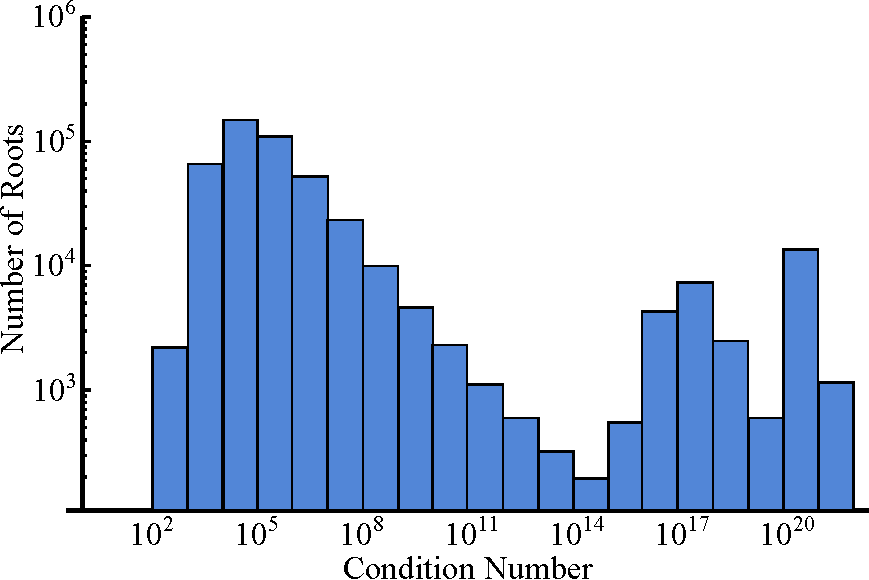
\includegraphics[scale=0.5]{root_histogram}
\caption{Condition numbers of Jacobian matrices at the solutions found during the leg mechanism example.  We assume solutions with condition numbers greater than $10^{15}$ are singular.}
\label{root_histogram}
\end{figure}

The system $\mathcal{S}(\mathbf{z},\mathbf{q}_\text{task})=0$ was solved by setting up a parameter homotopy with the ab initio roots as startpoints.
However, instead of computing 1,528,608 paths, one root from each cognate set was tracked, cutting this number in half.
Only one root is needed to establish its cognate set of roots of the target system at the end of a homotopy.
The parameter homotopy had a higher path failure rate of 41\%.  Of these failures, 91\% were triggered by the Jacobian condition number rising above $10^{18}$ which occurred on average at $t=0.997$ ($\pm 0.037$ S.D.).
Although it is not certain, this is an indicator that those paths might have been headed toward singular endpoints, which generally are not useful for engineering applications.
Singular endpoints are usually more common when $\mathcal{S}$ is defined with additional structure, such as the case with $\mathbf{q}_\text{task}$.
A histogram of endpoint condition numbers is shown in Fig. \ref{root_histogram}.  Informed by this, we chose a condition number of $10^{15}$ to separate endpoints considered nonsingular and singular.




There were 419,576 nonsingular cognate pairs of roots found.
A subset $\Omega$ of size 1861 were physically relevant, that is when variables and their overbar counterparts, e.g. $(A,\*A)$, are conjugate.
Recall from Section \ref{sec:cognates} that when parameters $Q_j$ and $\*Q_j$ are reciprocal, such as with the members of $\Omega$, the cognate operator $\kappa_{3/4}$ extends the cognate sets from size two to four.
Therefore, we should expect the cognate pairs of $\Omega$ to divide into half as many cognate foursomes.
However, $1861/2\notin\mathbb{N}$, indicating a problem.
Sorting out $\Omega$, we instead found 920 cognate foursomes and 21 incomplete cognate pairs.
Missing cognates were most likely lost during numerical work, but are readily producible in post-process using the cognate transforms of Section \ref{sec:cognates}.
Expanding out all 941 cognate foursomes obtains 3764 linkage designs.


\begin{figure}[!t]
\centering
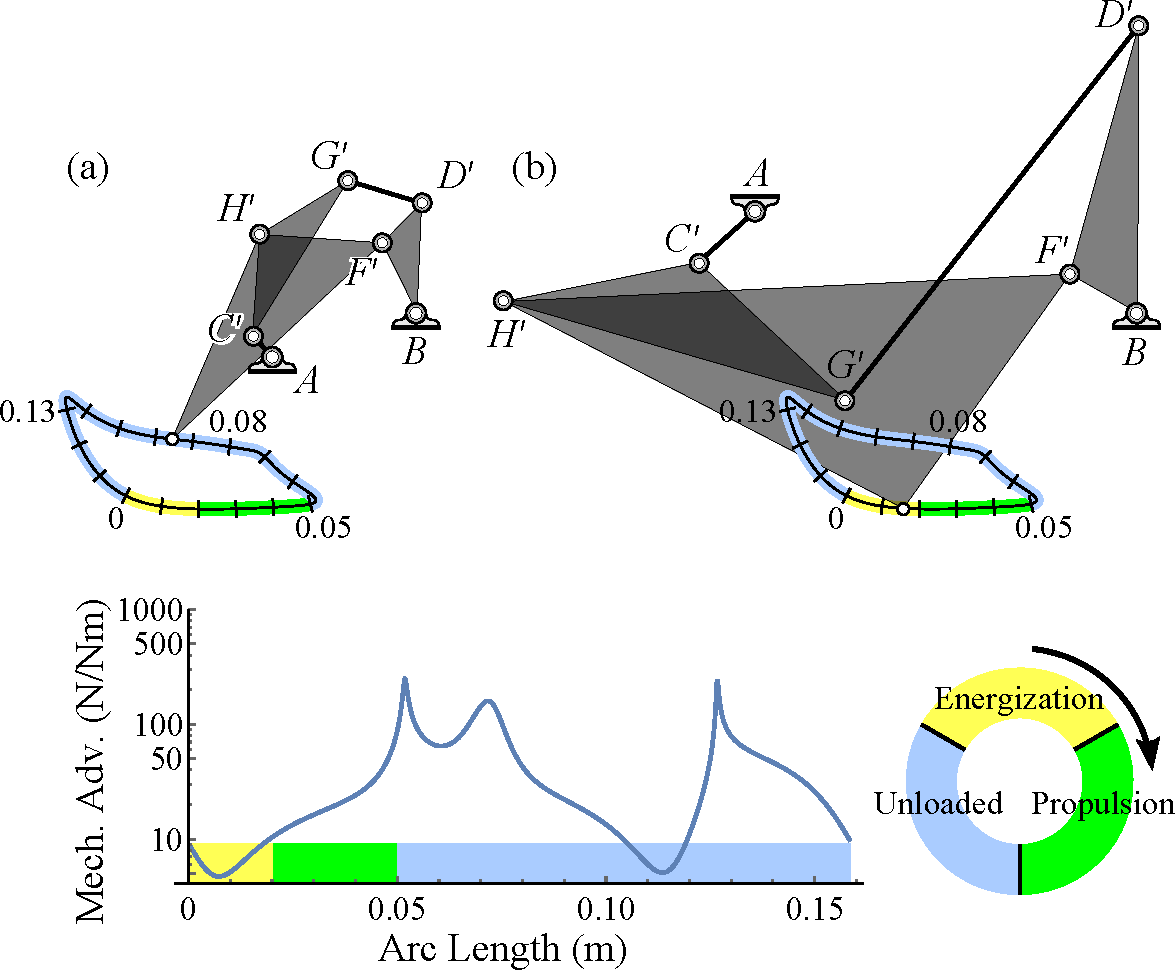
\includegraphics[scale=0.4]{synth_results_first}
\hfil
\vspace{5mm}
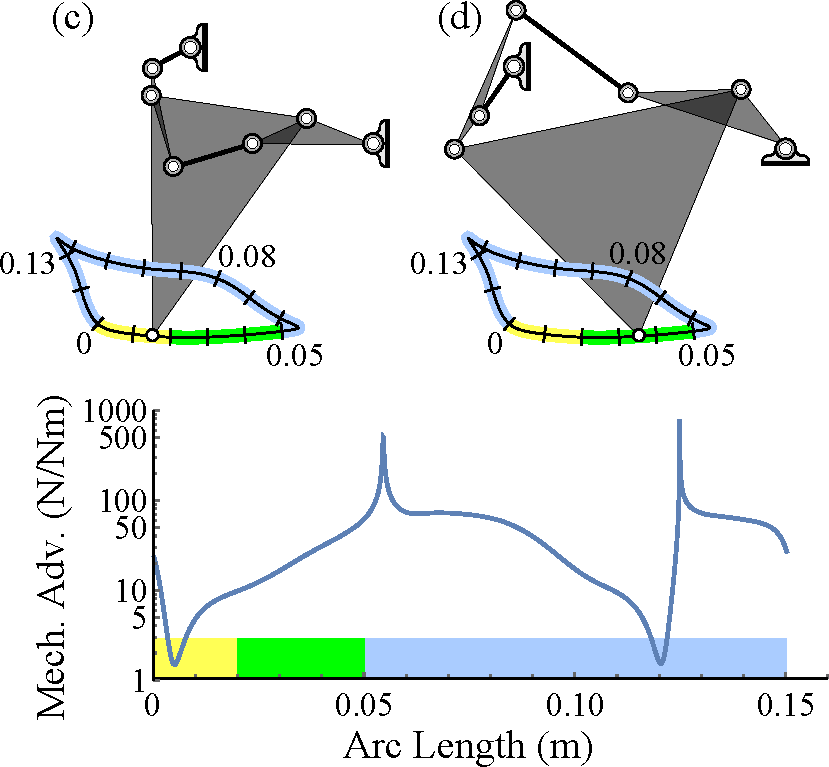
\includegraphics[scale=0.4]{synth_results_second}
\caption{Linkage designs that exhibit the desired dynamic behavior.  Linkages (a) and (b) are cognates that trace the exact same path with the same coordination of mechanical advantage over arclength.  The same goes for (c) and (d).}
\label{synth_results}
\end{figure}


These linkage designs are susceptible to a known list of linkage defects: circuit, branch, order, and full rotatability defects \cite{balliDefectsLinkMechanisms2002}.
To sort these out, all designs were kinematically analyzed.
Occasionally designs were found to possess circuit defects but were still deemed useful.
That is, if a mechanism circuit missed one or two task points but still approximated the motion that $\mathbf{q}_\text{task}$ was chosen to approximate in the first place, that mechanism was considered useful.
In addition, linkages must have pivots in acceptable locations (e.g. not underground) and ideally be compact.
A few linkage designs which satisfy these criteria are drawn in Fig. \ref{synth_results}.
The linkages shown in Figs. \ref{synth_results}a and \ref{synth_results}b are cognates.  Likewise with \ref{synth_results}c and \ref{synth_results}d.
That being the case, they produce the same point path with the same variation of mechanical advantage across that path.
Therefore, the plots printed under each pair in Fig. \ref{synth_results} describe both linkages above.


\begin{figure}[!t]
\centering
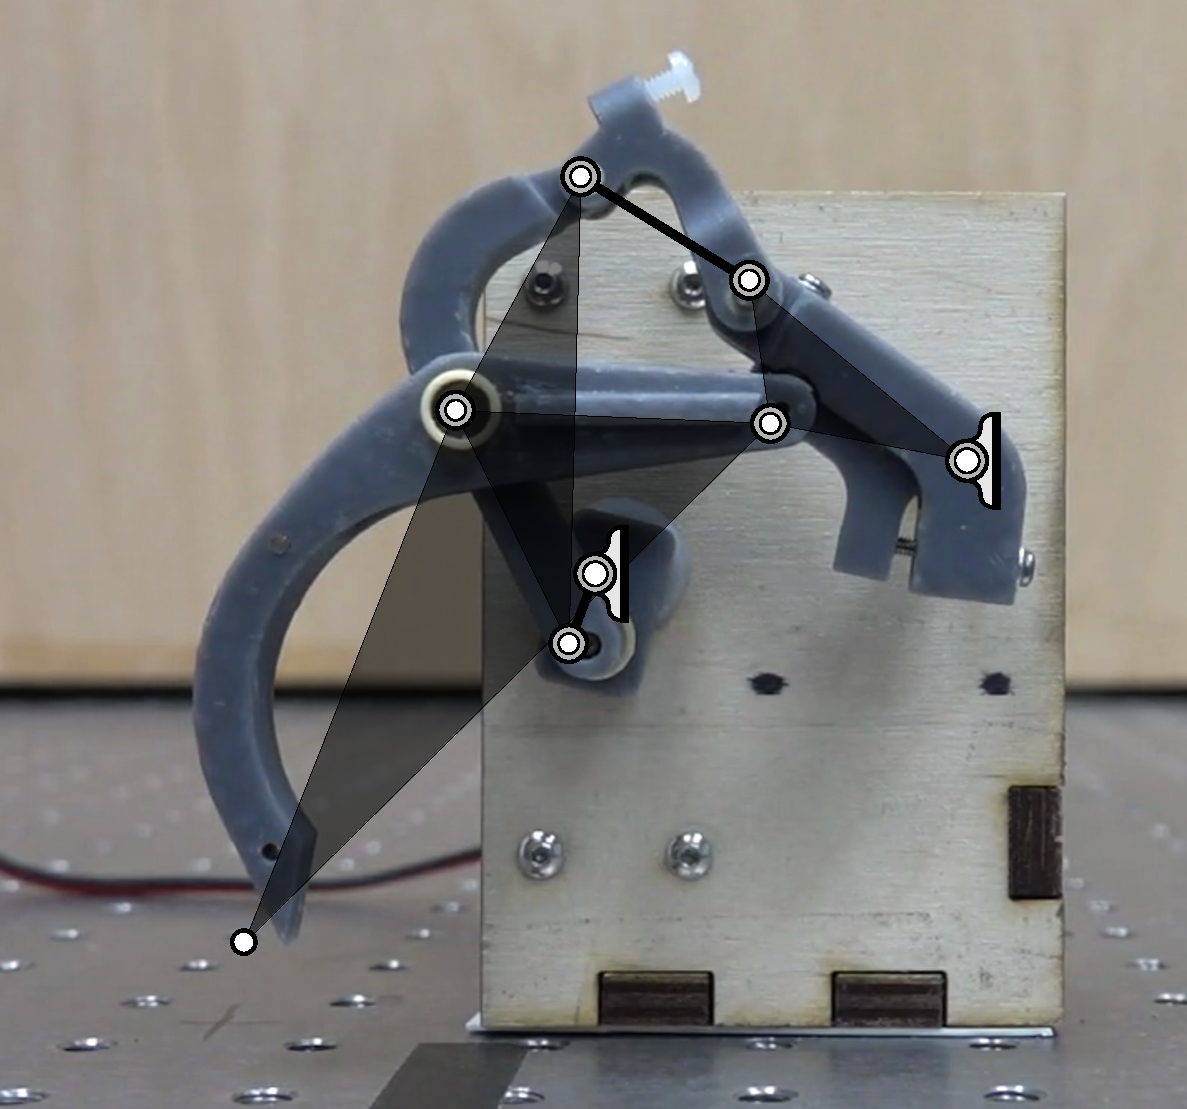
\includegraphics[scale=0.3]{prototype_overlay}
\caption{The linkage drawn in Fig. \ref{synth_results}a was constructed.}
\label{prototype_overlay}
\end{figure}



\begin{figure}[!t]
\centering
%\subfloat[]{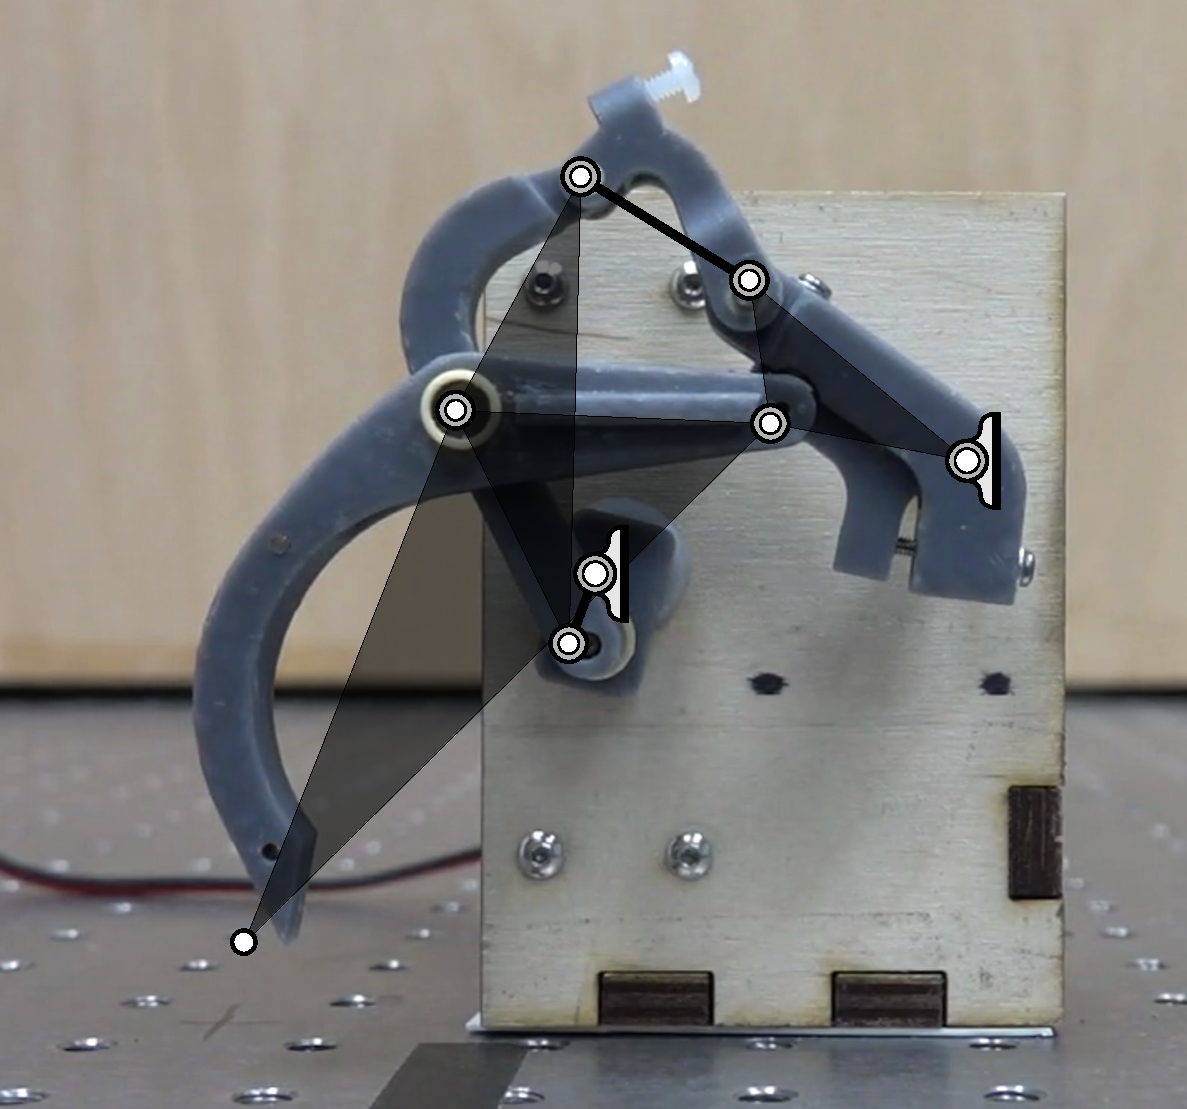
\includegraphics[scale=0.3]{prototype_overlay}%
%\label{prototype_overlay}}
%\hfil
\subfloat[]{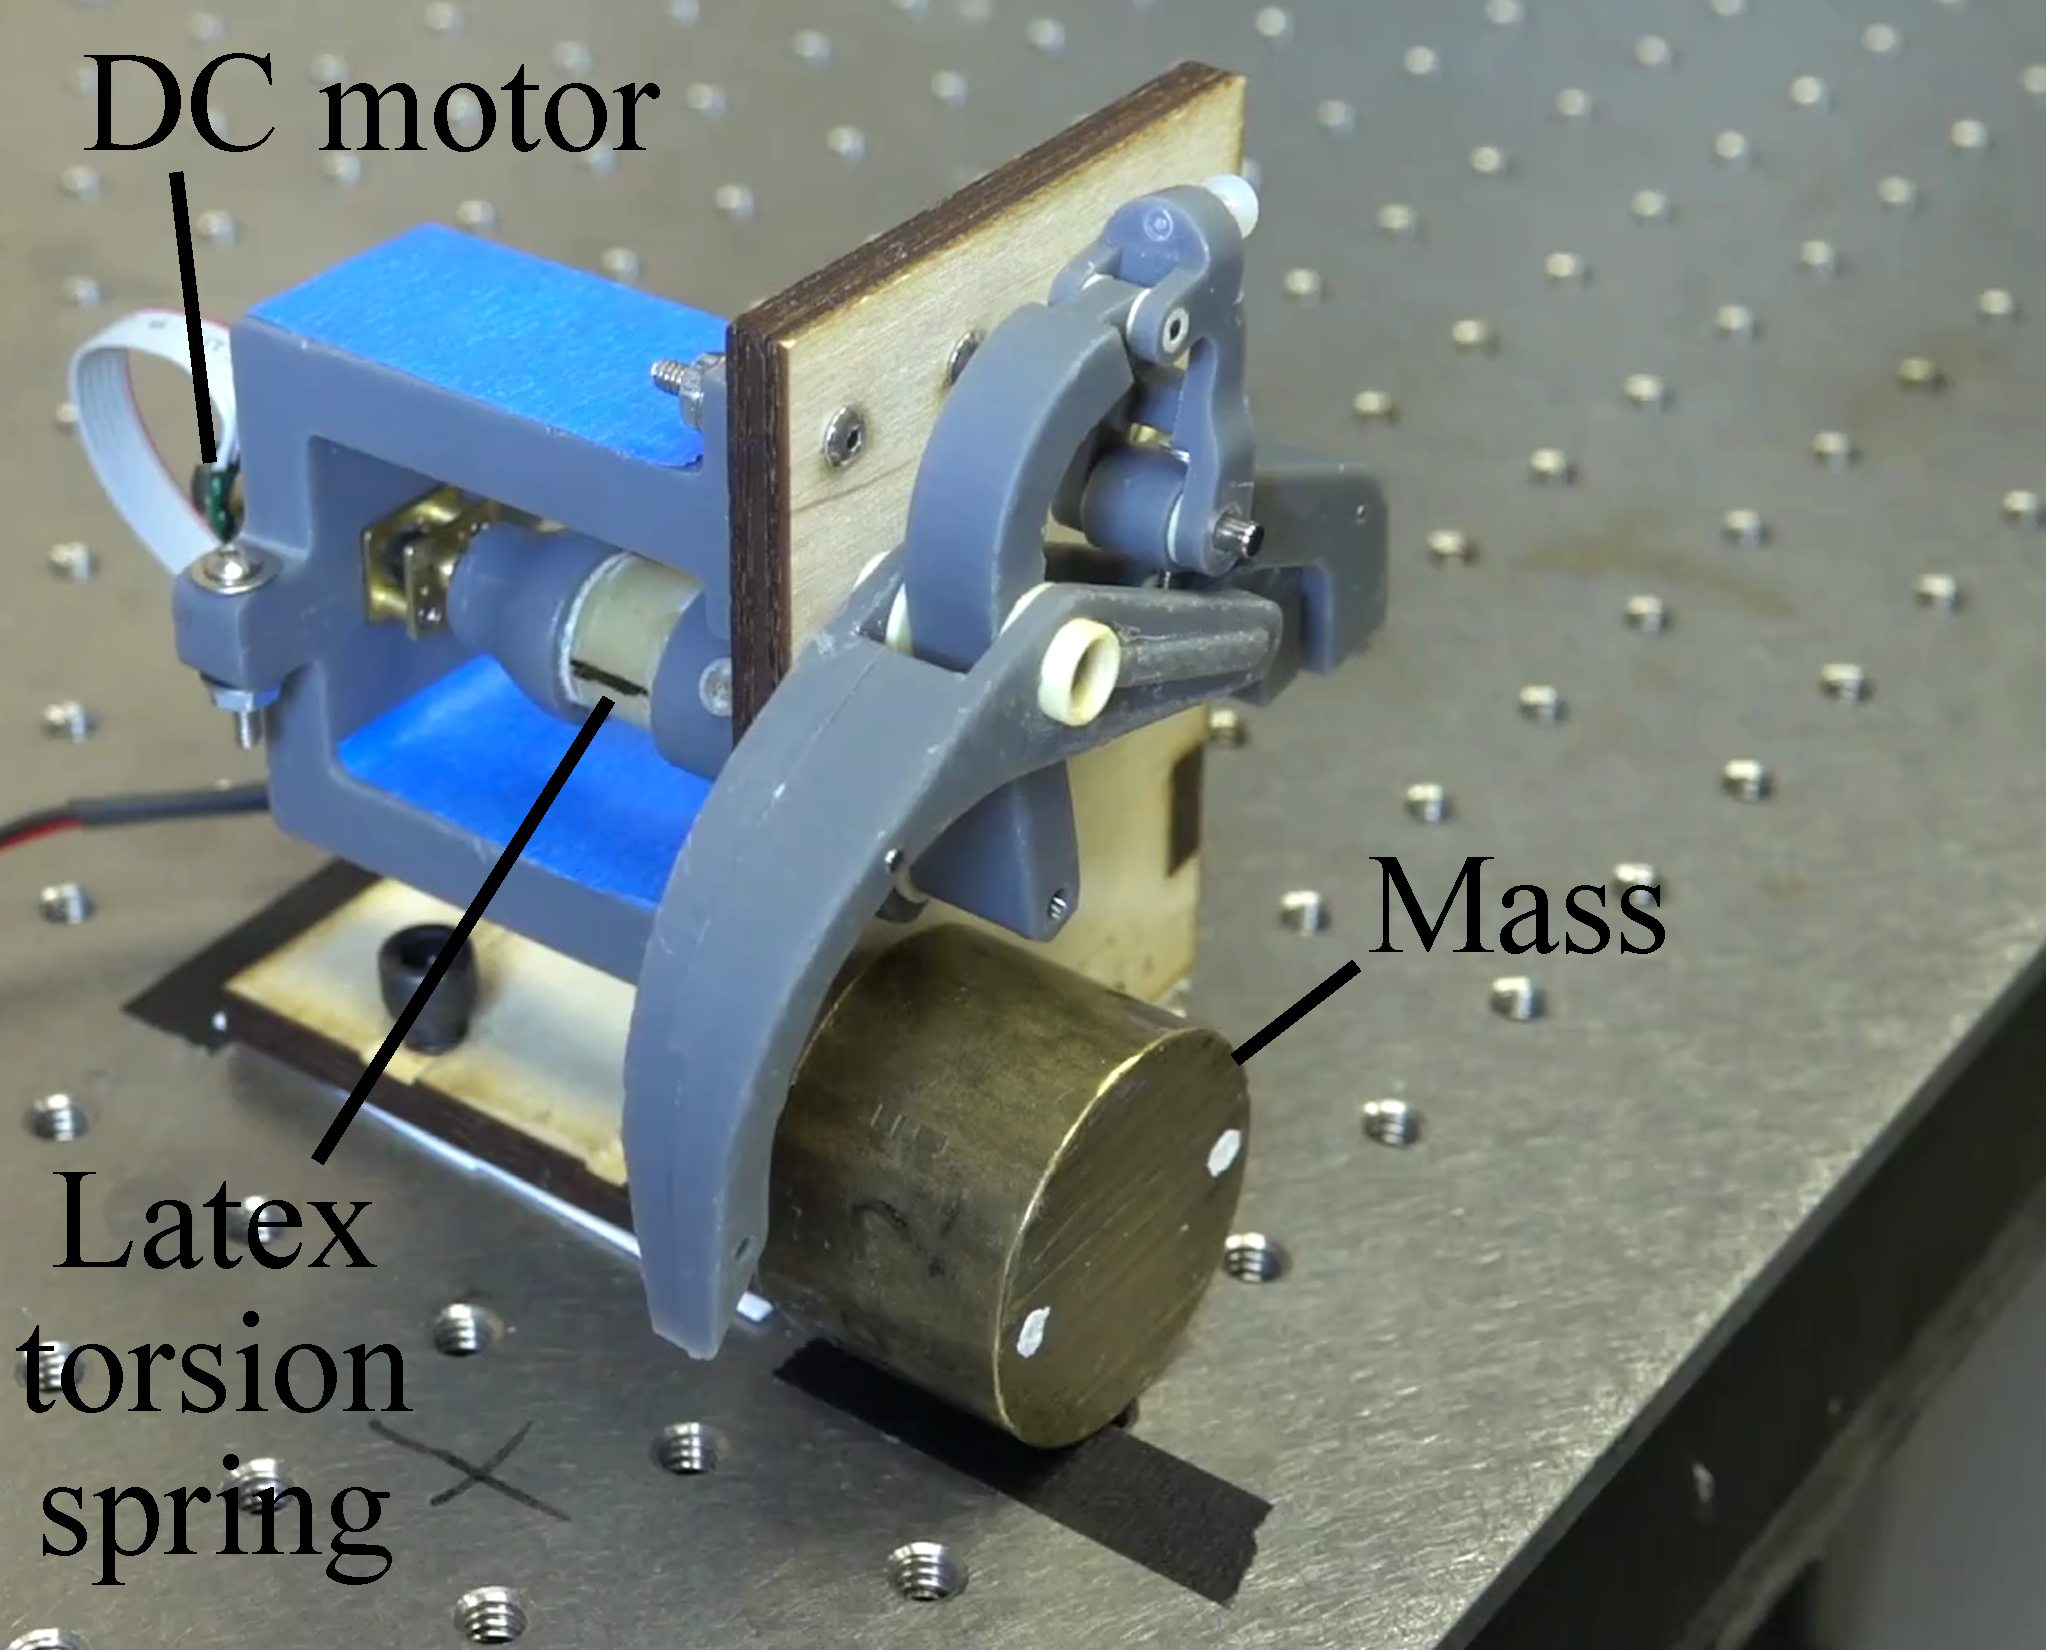
\includegraphics[scale=0.12]{prototype_ready}%
\label{prototype_ready}}
\hfil
\subfloat[]{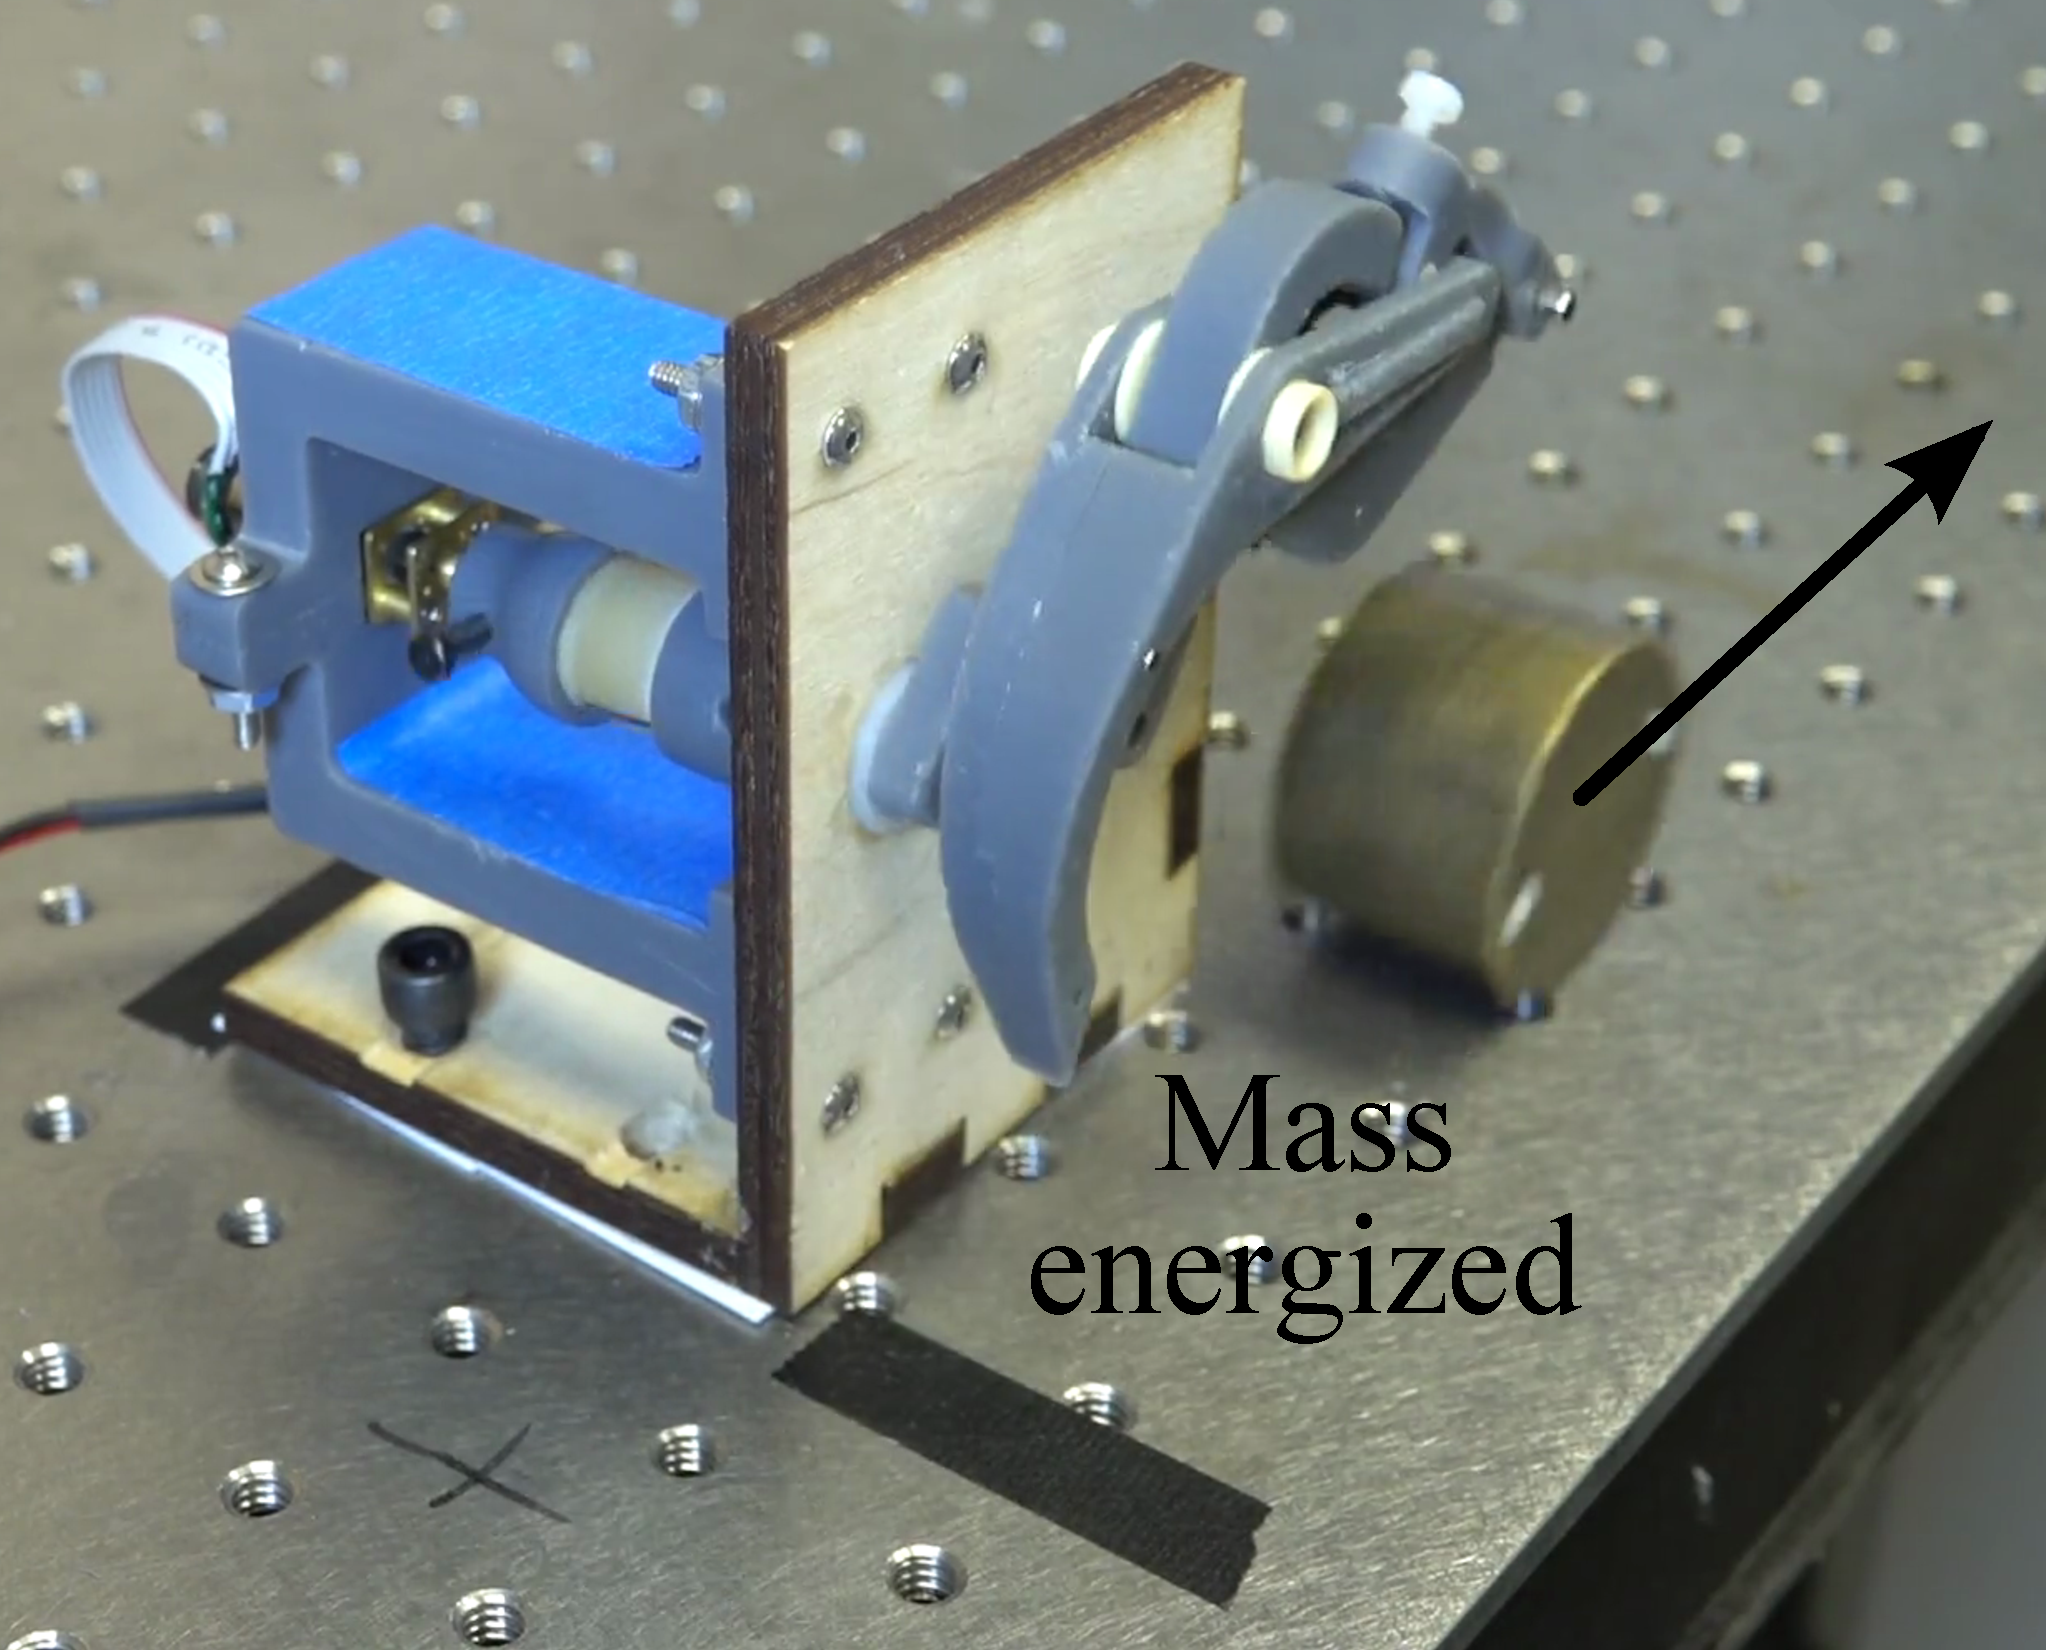
\includegraphics[scale=0.12]{prototype_rolling}%
\label{prototype_rolling}}
\caption{The constructed linkage was connected to a series-elastic actuator (specs in Table \ref{simulation_parameters}).  An experiment similar to the mock-up dynamic model of Fig. \ref{dynamic_model} was carried out.}
\label{prototype_experiment}
\end{figure}


The cycling foot path is broken into three regions.  
First, the foot point makes ground contact and mechanical advantage decreases, nearly stalling motion and energizing the series-elastic element.
Second, while still in stance mechanical advantage increases, converting elastic energy into high-powered propulsion.
And third, the foot goes out of contact and recycles back to its starting position.
Although only a single low mechanical advantage region was desired, a second is seen in the unloaded regions of Fig. \ref{synth_results}.
It was common to nearly all designs that had the foot path entirely below the ground pivots, that installing a low mechanical advantage region on one part of the curve begot another low mechanical advantage region elsewhere.
It is unclear whether it is possible to exclude this second region and maintain pivots above the foot path.
This just might be the circumstance of the design space we are navigating.
Anyway, as the second low spot appears in the unloaded region, it is not problematic.




%These points may be taken unaltered or modified using local optimization.
%Simulation ensures designs produce the desired dynamic behavior.









To validate design results, the solution drawn in Fig. \ref{synth_results}a was built and tested, pictured in Fig. \ref{prototype_overlay}.
More extensive test results are presented in \cite{plecnikAdjustablePowerModulation2019}.
The prototype consists of a 1 W Pololu motor that twists a torsion spring (cylindrical cut of latex) which rotates the input crank of a 3D printed linkage mounted to a wooden board.
An experiment was set up similar to the dynamics illustrated in Fig. \ref{dynamic_model} where the leg mechanism pushes a weight.
The leg was able to modulate mechanical power 2.6 times beyond the motor's output.
Simulation indicated a factor of 3.0 times could be possible.
Sources of energy loss include the movement of unaccounted link inertias and friction.




% An example of a floating figure using the graphicx package.
% Note that \label must occur AFTER (or within) \caption.
% For figures, \caption should occur after the \includegraphics.
% Note that IEEEtran v1.7 and later has special internal code that
% is designed to preserve the operation of \label within \caption
% even when the captionsoff option is in effect. However, because
% of issues like this, it may be the safest practice to put all your
% \label just after \caption rather than within \caption{}.
%
% Reminder: the "draftcls" or "draftclsnofoot", not "draft", class
% option should be used if it is desired that the figures are to be
% displayed while in draft mode.
%
%\begin{figure}[!t]
%\centering
%\includegraphics[width=2.5in]{myfigure}
% where an .eps filename suffix will be assumed under latex, 
% and a .pdf suffix will be assumed for pdflatex; or what has been declared
% via \DeclareGraphicsExtensions.
%\caption{Simulation results for the network.}
%\label{fig_sim}
%\end{figure}

% Note that the IEEE typically puts floats only at the top, even when this
% results in a large percentage of a column being occupied by floats.


% An example of a double column floating figure using two subfigures.
% (The subfig.sty package must be loaded for this to work.)
% The subfigure \label commands are set within each subfloat command,
% and the \label for the overall figure must come after \caption.
% \hfil is used as a separator to get equal spacing.
% Watch out that the combined width of all the subfigures on a 
% line do not exceed the text width or a line break will occur.
%
%\begin{figure*}[!t]
%\centering
%\subfloat[Case I]{\includegraphics[width=2.5in]{box}%
%\label{fig_first_case}}
%\hfil
%\subfloat[Case II]{\includegraphics[width=2.5in]{box}%
%\label{fig_second_case}}
%\caption{Simulation results for the network.}
%\label{fig_sim}
%\end{figure*}
%
% Note that often IEEE papers with subfigures do not employ subfigure
% captions (using the optional argument to \subfloat[]), but instead will
% reference/describe all of them (a), (b), etc., within the main caption.
% Be aware that for subfig.sty to generate the (a), (b), etc., subfigure
% labels, the optional argument to \subfloat must be present. If a
% subcaption is not desired, just leave its contents blank,
% e.g., \subfloat[].


% An example of a floating table. Note that, for IEEE style tables, the
% \caption command should come BEFORE the table and, given that table
% captions serve much like titles, are usually capitalized except for words
% such as a, an, and, as, at, but, by, for, in, nor, of, on, or, the, to
% and up, which are usually not capitalized unless they are the first or
% last word of the caption. Table text will default to \footnotesize as
% the IEEE normally uses this smaller font for tables.
% The \label must come after \caption as always.
%
%\begin{table}[!t]
%% increase table row spacing, adjust to taste
%\renewcommand{\arraystretch}{1.3}
% if using array.sty, it might be a good idea to tweak the value of
% \extrarowheight as needed to properly center the text within the cells
%\caption{An Example of a Table}
%\label{table_example}
%\centering
%% Some packages, such as MDW tools, offer better commands for making tables
%% than the plain LaTeX2e tabular which is used here.
%\begin{tabular}{|c||c|}
%\hline
%One & Two\\
%\hline
%Three & Four\\
%\hline
%\end{tabular}
%\end{table}



\section{Conclusion}
\label{sec:conclusion}


The conclusion goes here.


\appendices
\section{Fourier Coefficients}
\label{app:fourier_coefficients}

\vspace{2mm}

Fourier coefficients for example's path

\vspace{2mm}

%\begin{table}[h]
%\caption{Fourier coefficients for example's path}
%\label{table_example}
%\centering
\noindent
\resizebox{80mm}{!}{%
\begin{tabular}{|c|rrrr|}
\hline
$k$ & \multicolumn{1}{c}{$a_k$} & \multicolumn{1}{c}{$b_k$} & \multicolumn{1}{c}{$c_k$} & \multicolumn{1}{c|}{$d_k$} \\
\hline
0 & 5.0380E-02 &   & 1.0006E-02 &  \\
1 & -2.3035E-02 & 8.1134E-03 & -3.3929E-04 & -9.9926E-03 \\
2 & 1.4741E-04 & -7.4818E-04 & -1.9118E-03 & -1.2695E-03 \\
3 & -9.8067E-04 & 1.7724E-03 & -1.2544E-03 & -5.7305E-04 \\
4 & -1.4305E-04 & -6.3621E-04 & -4.2266E-04 & 2.5945E-04 \\
5 & 6.9575E-05 & 3.8911E-04 & -3.7591E-04 & 1.0048E-04 \\
6 & -3.8162E-04 & -2.8942E-04 & 2.5620E-05 & 5.2924E-05 \\
7 & 8.3483E-05 & 5.0805E-05 & -8.7071E-05 & 6.9878E-05 \\
\hline
\end{tabular}
}
%\end{table}

\vspace{6mm}

Fourier coefficients for example's mechanical advantage

\vspace{2mm}

%\begin{table}[h]
%\caption{Fourier coefficients for example's mechanical advantage}
%\label{table_example}
%\centering
\noindent
\resizebox{1\linewidth}{!}{%
\begin{tabular}{|c|rr|c|rr|}
\hline
$k$ & \multicolumn{1}{c}{$\alpha_k$} & \multicolumn{1}{c|}{$\beta_k$} & $k$ & \multicolumn{1}{c}{$\alpha_k$} & \multicolumn{1}{c|}{$\beta_k$} \\
\hline
0 &  \multicolumn{1}{c}{4$\pi$} &   &   &   &  \\
1 & -3.3934E+00 & -4.3419E+00 & 9 & 1.3074E-01 & 3.7434E-02 \\
2 & -6.0540E-01 & -8.4776E-01 & 10 & 9.7375E-02 & 2.8083E-03 \\
3 & -9.5055E-01 & 8.3538E-02 & 11 & 7.1065E-02 & -7.1290E-02 \\
4 & -4.9012E-01 & 3.8890E-02 & 12 & 3.5888E-02 & -6.8938E-02 \\
5 & -2.7556E-01 & 3.2529E-01 & 13 & -2.9838E-02 & -5.8048E-02 \\
6 & -1.4824E-01 & 2.4851E-01 & 14 & -3.3223E-02 & -4.2639E-02 \\
7 & 6.3071E-02 & 2.2760E-01 & 15 & -4.6873E-02 & 9.3571E-03 \\
8 & 8.9012E-02 & 1.3820E-01 & 16 & -3.7274E-02 & -4.0571E-03 \\
\hline
\end{tabular}
}
%\end{table}


\section{Forward Kinematics}
\label{app:fwd_kin}

The forward kinematics as solved for generating startpoints and start systems in Section \ref{sec:start_sys} are given here.
Notation follows the definitions already given in Section \ref{sec:synth_eq} and Fig. \ref{synthesis_diagram}.

The geometric input parameter for this single degree-of-freedom linkage is the value of $\rho-\mu$.

First, consider the floating four-bar $DGHF$ characterized by the loop equation
\begin{equation}
T(G-D) + R(H-G) - U(H-F) = S(F-D). \label{four-bar_loop}
\end{equation}
Multiplying Eqn. (\ref{four-bar_loop}) by $\*U$ obtains
\begin{equation}
T\*U(G-D) + R\*U(H-G) - H+F = S\*U(F-D). \label{TUloop}
\end{equation}
Values of $R\*U$ are the geometric input,
\begin{equation}
R\*U = e^{i(\rho-\mu)}
\end{equation}
Relative rotation operator $S\*U$ may be eliminated by multiplying Eqn. (\ref{TUloop}) by its conjugate,
\begin{equation}
\mathcal{A}_\text{I} T\*U + \*{\mathcal{A}}_\text{I} \*TU + \mathcal{B}_\text{I} = 0,
\label{quadratic1}
\end{equation}
where
\begin{align}
\mathcal{A}_\text{I} &= (G-D) \Big( \frac{1}{R\*U} (\*H-\*G) - \*H+\*F) \Big), \\[1mm]
\*{\mathcal{A}}_\text{I} &= (\*G-\*D) \Big( R\*U(H-G) - H+F) \Big), \nonumber\\
\mathcal{B}_\text{I} &= R\*U(H-G)(\*H-\*F) - \frac{1}{R\*U}(\*H-\*G)(H-F) \nonumber\\
&\hspace{5mm} + (G-D)(\*G-\*D) + (H-G)(\*H-\*G) \nonumber\\
&\hspace{5mm} + (H-F)(\*H-\*F) - (F-D)(\*F-\*D). \nonumber
\end{align}
Solving Eqn. (\ref{quadratic1}) for $T\*U$ obtains
\begin{equation}
T\*U = \frac{1}{2\mathcal{A}}\left( -\mathcal{B} \pm \sqrt{\mathcal{B}^2 - 4\mathcal{A}\*{\mathcal{A}} }\; \right)
\end{equation}
Note the ``$\pm$'' operator.
For generating a startpoint/start system in Section \ref{sec:start_sys}, either the ``$+$'' or ``$-$'' solution is randomly selected.
With values $R\*U$ and $T\*U$ known, the value of $S\*U$ may be obtained simply from Eqn. (\ref{TUloop}).

Next, we consider the five-bar $ACGDB$ with loop equation,
\begin{align}
A-B + R(H-C) - S(F-B) - \nonumber\\
U(H-F) = -Q(C-A). \label{five-bar_loop}
\end{align}
Multiplying Eqn. (\ref{five-bar_loop}) by $\*U$ obtains,
\begin{align}
\*U(A-B) + R\*U(H-C) - S\*U(F-B) - \nonumber\\
H+F = -Q\*U(C-A) \label{Uloop}
\end{align}
Values of $R\*U$ and $S\*U$ are already known.  
Relative rotation operator $Q\*U$ may be eliminated by multiplying Eqn. (\ref{Uloop}) by its conjugate,
\begin{equation}
\mathcal{A}U + \*{\mathcal{A}}\*U + \mathcal{B} = 0, \label{quadratic2}
\end{equation}
where
\begin{align}
\mathcal{A} &= (\*A-\*B) \Big( R\*U(H-C) - S\*U(F-B) - H+F \Big), \nonumber\\
\*{\mathcal{A}} &= (A-B) \Big( \frac{1}{R\*U}(\*H-\*C) - \frac{1}{S\*U}(\*F-\*B) - \*H+\*F \Big), \nonumber\\[1mm]
\mathcal{B} &= \Big( R\*U(H-C) - S\*U(F-B) - H+F \Big) \times \nonumber\\
&\hspace{5mm} \Big( \frac{1}{R\*U}(\*H-\*C) - \frac{1}{S\*U}(\*F-\*B) - \*H+\*F \Big) + \nonumber\\
&\hspace{5mm} (A-B)(\*A-\*B) - (C-A)(\*C-\*A)
\end{align}
Solving Eqn. (\ref{quadratic2}) for $U$ obtains
\begin{equation}
U = \frac{1}{2\mathcal{A}}\left( -\mathcal{B} \pm \sqrt{\mathcal{B}^2 - 4\mathcal{A}\*{\mathcal{A}} }\; \right)
\end{equation}
Just as earlier, either the ``$+$'' or ``$-$'' is randomly selected.
With values $R\*U$, $S\*U$, and $\*U = 1/U$ all known, the value of $Q\*U$ may be obtained simply from Eqn. (\ref{Uloop}).

Now values of $Q$, $R$, $S$, $T$, are simply obtained from values of their relative angle counterparts,
\begin{align}
Q &= Q\*U \times U, & R &= R\*U \times U, \nonumber\\
S &= S\*U \times U, & T &= T\*U \times U.
\end{align}
The end effector point $P$ is located at
\begin{equation}
P = B + S(F-B) + U(P_0-F).
\end{equation}
Values of $U$, $Q$, and $P$ are used to complete vectors $\mathbf{z}$ and $\mathbf{q}$ in Section \ref{sec:start_sys}, defining a startpoint and start system.


\section{Target Parameters}
\label{app:fpm}

%\begin{table}[h]
%\caption{Fourier Coefficients for Example Path}
%\label{final_parameters}
%\centering
\noindent
\resizebox{1\linewidth}{!}{%
\begin{tabular}{@{\;}r@{}r@{}l@{\;}|@{\;}r@{}r@{}l@{\;}}
%\hline
$P_0$ = & 4.241713408    & $-$4.925334736$i$ & $\*P_0$ = & $-$3.76987048 & $+$0.79723779$i$ \\
$P_1$ = & 1.448005491    & $-$2.686249989$i$ & $\*P_1$ = & $-$4.28563116 & $-$0.56502469$i$ \\
$P_2$ = & 2.287911195    & $-$0.912310849$i$ & $\*P_2$ = & $-$2.16603080 & $+$0.88360558$i$ \\
$P_3$ = & $-$1.870502484 & $-$0.577807741$i$ & $\*P_3$ = & 4.57926095    & $-$2.07401374$i$ \\
$P_4$ = & $-$0.762532942 & $+$0.904378820$i$ & $\*P_4$ = & 4.80128973    & $-$1.46072184$i$ \\
$P_5$ = & $-$4.142822754 & $+$1.697671323$i$ & $\*P_5$ = & 2.04126667    & $+$2.96214923$i$ \\
$P_6$ = & 1.023004534    & $-$3.026210036$i$ & $\*P_6$ = & 3.98999969    & $-$0.23282959$i$ \\
$P_7$ = & $-$2.522295756 & $+$3.942421532$i$ & $\*P_7$ = & $-$3.99644836 & $+$4.42685486$i$ \\
$Q_1$ = & 2.315936720    & $-$0.552780386$i$ & $\*Q_1$ = & $-$0.21802981 & $+$3.58500421$i$ \\
$Q_2$ = & $-$3.018911858 & $+$0.969238414$i$ & $\*Q_2$ = & 4.31106320    & $-$0.03375595$i$ \\
$Q_3$ = & $-$0.490634736 & $+$2.994316904$i$ & $\*Q_3$ = & 4.93814807    & $+$4.55170197$i$ \\
$Q_4$ = & 0.239711851    & $-$1.341440198$i$ & $\*Q_4$ = & $-$4.27121444 & $+$0.13553499$i$ \\
$Q_5$ = & 4.942917423    & $-$2.415216683$i$ & $\*Q_5$ = & $-$0.73774348 & $+$1.83173884$i$ \\
$Q_6$ = & 1.599536874    & $+$2.367319121$i$ & $\*Q_6$ = & 0.88946147    & $+$0.86574737$i$ \\
$Q_7$ = & 4.229853181    & $-$1.149104288$i$ & $\*Q_7$ = & 4.03675786    & $+$1.46116468$i$ \\
%\hline
\end{tabular}
}
%\end{table}



\section{Homotopy Path Tracking}
\label{app:tracking}

Here we present a method for tracking the homotopy paths of a system $\mathbf{f}(\mathbf{z},\mathbf{q})=0$.  The vector of variables $\mathbf{z}$ has $n$ components, and the vector of parameters $\mathbf{q}$ has $m$ components.
We define parameters for a start system and target system as $\mathbf{q}_0$ and $\mathbf{q}_1$, respectively.
Our goal is to track the values of a root $\mathbf{z}$ from a startpoint $\mathbf{z}=\mathbf{z}_0$ that solves the start system $\mathbf{f}(\mathbf{z},\mathbf{q}_0) = 0$ to an endpoint $\mathbf{z}=\mathbf{z}_1$ that solves the target system $\mathbf{f}(\mathbf{z},\mathbf{q}_1) = 0$.
To do this, we construct a homotopy parameterized by $t$,
\begin{align}
&\mathbf{f}(\mathbf{z},\mathbf{q}(t)) = 0 \label{homotopy}\\
&\text{where} \quad \mathbf{q}(t) = \dfrac{\gamma(1-t)\mathbf{q}_0 + t\mathbf{q}_1}{\gamma(1-t) + t}.
\end{align}
The definition of $\mathbf{q}(t)$ follows the ``gamma trick'' \cite{batesNumericallySolvingPolynomial2013}.  At $t=0$, Eqn. (\ref{homotopy}) is the start system.  At $t=1$, it is the target system.

In order to gain some numerical benefits \cite{morganHomotopySolvingGeneral1987}, path tracking is done in projective space.
Therefore, we define homogeneous coordinates of $\mathbf{z}$ as
\begin{equation}
\mathbf{Z} = [ Z_1, \ldots, Z_n, Z_0 ] \quad \text{where} \quad 
\begin{Bmatrix} \mathbf{z} \\ 1 \end{Bmatrix} = \mathbf{Z}/Z_0.
\end{equation}
The modified version of $\mathbf{f}$ that receives $\mathbf{Z}$ as an argument is named $\mathbf{F}$.
A linear patch is needed for projective computations, defined as
\begin{equation}
\mathbf{u} \cdot \begin{Bmatrix} \mathbf{Z} \\ t \end{Bmatrix}  - 1 = 0,
\label{patch}
\end{equation}
where $\mathbf{u}$ is an $n+2$ dimensional vector of random complex coefficients.
Repackaging $\mathbf{Z}$ and $t$ into a single vector $\mathbf{Y} = \{ \mathbf{Z}, t \}$, the homotopy is written as
\begin{equation}
\mathbf{H}(\mathbf{Y}) = 
\begin{Bmatrix} 
\mathbf{F}(\mathbf{Z}, \mathbf{q}(t)) \\ 
\mathbf{u}\cdot\mathbf{Y} -1
\end{Bmatrix}= 0 \label{homotopy_projected}
\end{equation}
$\mathbf{Y}$ may be considered a function of the homotopy path's arclength $s$. Taking the derivative of $\mathbf{H}$ with respect to $s$ obtains
\begin{equation}
\left[ \frac{\partial \mathbf{H}}{\partial \mathbf{Y}} \right] \frac{d\mathbf{Y}}{ds} = 0. \label{homotopy_derivative}
\end{equation}
Expansion of the Jacobian matrix on the left side of Eqn. (\ref{homotopy_derivative}) obtains
\begin{align}
\left[ \frac{\partial \mathbf{H}}{\partial \mathbf{Y}} \right] = 
&\left[\begin{array}{cc}
\left[ \frac{\partial \mathbf{F}}{\partial \mathbf{Z}} \right] & 
\frac{d\mathbf{F}}{dt} \label{Jacobian_expansion}\\[2mm]
\multicolumn{2}{c}{\cdots\mathbf{u}^\text{T}\cdots}
\end{array} \right], \\[2mm]
\text{where} \quad &\frac{d\mathbf{F}}{dt} = \left[ \frac{\partial \mathbf{F}}{\partial \mathbf{q}} \right] \frac{d\mathbf{q}}{dt}, \nonumber\\[1mm]
\text{and} \quad &\frac{d\mathbf{q}}{dt} = (\mathbf{q}_1 - \mathbf{q}_0)\frac{\gamma}{\big( \gamma(1-t)+t \big)^2}. \nonumber
\end{align}
\medmuskip=1mu
In Eqn. (\ref{Jacobian_expansion}), $\left[ \frac{\partial \mathbf{H}}{\partial \mathbf{Y}} \right]$ is an $(n+1) \times (n+2)$ matrix, $\left[ \frac{\partial \mathbf{F}}{\partial \mathbf{Z}} \right]$ is an $n \times (n+1)$ matrix, $\frac{d\mathbf{F}}{dt}$ is an $n \times 1$ vector, $\left[ \frac{\partial \mathbf{F}}{\partial \mathbf{q}} \right]$ is an $n \times m$ matrix, $\frac{d\mathbf{q}}{dt}$ is an $m \times 1$ vector, and $\mathbf{u}^\text{T}$ is a $1 \times (n+2)$ row vector.
\medmuskip=4mu

%For brevity, we rewrite Eqn. xx as
%\begin{equation}
%[J(\mathbf{Y})]\mathbf{Y}' = 0.
%\end{equation}
%

At a given point on a homotopy path, the vector space tangent to the path may be obtained by solving for $\frac{d\mathbf{Y}}{ds}$ in the homogeneous linear system given in Eqn. (\ref{homotopy_derivative}).
Note that the row vectors of $\left[ \frac{\partial \mathbf{H}}{\partial \mathbf{Y}} \right]$ are normal to the homotopy path so that the solutions of Eqn. (\ref{homotopy_derivative}) define the one dimensional vector space perpendicular to all $n+1$ normal vectors, i.e. tangent to the curve.
Numerically, Eqn. (\ref{homotopy_derivative}) is solved by appending a random row vector to $\left[ \frac{\partial \mathbf{H}}{\partial \mathbf{Y}} \right]$, appending 1 to the zero vector on the right hand side, then solving this square linear system.
For numerical stability, the appended row vector may be the tangent vector from the previous homotopy step.
The solution of this square system can be multiplied by complex scalars to achieve any vector in the $\mathbb{C}^1$ null space of $\left[ \frac{\partial \mathbf{H}}{\partial \mathbf{Y}} \right]$.
For the implementation given here, solutions were chosen to have unit magnitude and were scaled so that the last component of $\frac{d\mathbf{Y}}{ds}$ (corresponding to $t$) is a positive real number.


This solution process for discovering a tangent vector may be posed as an initial value problem, $\mathbf{Y}' = f(\mathbf{Y})$.
At the $i^\text{th}$ tracking step, a Runge-Kutta method can be applied to this initial value problem to compute from the current value $\mathbf{Y}_c$ an appropriate step size $\Delta s$, an estimate of the next value $\tilde{\mathbf{Y}}_n$, and a estimate of the next tangent vector $\tilde{\mathbf{V}}_n$.

This estimate is corrected by solving Eqn. (\ref{homotopy_projected}) with Newton's method using $\tilde{\mathbf{Y}}_n$ as the initial guess.  
Since Eqn. (\ref{homotopy_projected}) has one less equation than variables in $\mathbf{Y}$, we modify the process slightly.
An extra equation is appended to $\mathbf{H}(\mathbf{Y})$,
\begin{equation}
\hat{\mathbf{H}}(\mathbf{Y}) = 
\begin{Bmatrix}
\mathbf{H}(\mathbf{Y}) \\
\tilde{\mathbf{V}}_n \cdot (\mathbf{Y} - \delta \tilde{\mathbf{Y}}_n)
\end{Bmatrix} = 0 \label{homotopy_augmented}
\end{equation}
This is the equation of a plane nearly coincident to $\tilde{\mathbf{Y}}_n$ and normal to $\tilde{\mathbf{V}}_n$.  
The new variable $\delta$ is a small-valued complex scalar that serves as a correction factor to ensure an advancing value of $t$ is computed.
Assuming $\tilde{\mathbf{V}}_n$ is a good estimate of the homotopy path's tangent at the $i+1^\text{th}$ step, the intersection of the plane and path should be nearly perpendicular, aiding in numerical stability.

%To compute the $k+1^\text{th}$ Newton iteration, first evaluate

To compute the Newton iteration from $\mathbf{Y}_k$ to $\mathbf{Y}_{k+1}$, first evaluate the inverse of the Jacobian of (\ref{homotopy_augmented}) for $\mathbf{Y}_k$,
\begin{equation}
[\,\Gamma\,]_k = 
\begin{bmatrix}
\; \big[ \frac{\partial \mathbf{H}}{\partial \mathbf{Y}} \big]_k \; \\[2mm]
\tilde{\mathbf{V}}_n^\text{T}
\end{bmatrix}^{-1} \label{Jacobian_augmented}
\end{equation}
Note that $\delta$, which has not yet been evaluated, drops out of (\ref{Jacobian_augmented}).
To evaluate $\delta$, consider the Newton update rule
\begin{equation}
\mathbf{Y}_{k+1} = \mathbf{Y}_k - [\,\Gamma\,]_k \hat{\mathbf{H}}(\mathbf{Y}_k)
\label{Newton_update}
\end{equation}
The last component of Eqn. (\ref{Newton_update}) can be broken out and written
\begin{equation}
t_{k+1} = t_k - \mathbf{\Gamma}_{k,n+2} \cdot
\begin{Bmatrix}
\mathbf{H}(\mathbf{Y}_k) \\
\tilde{\mathbf{V}}_n \cdot (\mathbf{Y}_k - \delta \tilde{\mathbf{Y}}_n)
\end{Bmatrix} \label{last_row}
\end{equation}
where $\mathbf{\Gamma}_{k,n+2}$ is the last row of $[\,\Gamma\,]_k$.  At this point, everything in Eqn. (\ref{last_row}) has been numerically evaluated except $t_{k+1}$ and $\delta$.  
We set $t_{k+1}$ equal to the last component of $\tilde{\mathbf{Y}}_n$, then solve for $\delta$, which is straightforward.  
Now we are able to evaluate $\mathbf{Y}_{k+1}$ in Eqn. (\ref{Newton_update}) and Newton's method proceeds as usual.  
The value is converges to is the next homotopy path point $\mathbf{Y}_n$.  
An accurate tangent vector $\mathbf{V}_n$ is also produced by Newton's method.
The predictor-corrector path tracking process is repeated from these points.
When $t=1$ is reached, stop conditions for the Newton corrector are set to obtain more accurate solutions.

Occasionally, path tracking fails due to numerical precision limitations.
If this error is detected, the algorithm attempts to salvage the computation by switching projective linear patches, Eqn. (\ref{patch}), before reporting the failure.

To create a new patch, a vector $\mathbf{u}_\text{new}$ is randomly generated,
\begin{equation}
\mathbf{u}_\text{new} = \{ u_1 \; \ldots \; u_n \; u_0 \; u_t \}
\end{equation}
To continue computations, the vector of homogeneous coordinates $\mathbf{Z}$ must be multiplied by some scalar $\sigma$ so that it satisfies the new projective patch,
\begin{equation}
\mathbf{u}_\text{new} \cdot \begin{Bmatrix} \sigma\mathbf{Z} \\ t \end{Bmatrix}  - 1 = 0,
\label{new_patch}
\end{equation}
Solving Eqn. (\ref{new_patch}) for $\sigma$ obtains
\begin{equation}
\sigma = \frac{1 - u_t t}{\mathbf{u}_\text{new} \cdot \begin{Bmatrix} \mathbf{Z} \\ 0 \end{Bmatrix}}
\end{equation}
Tracking continues with $\mathbf{Y}$ replaced with $\mathbf{Y}_\text{new} = \begin{Bmatrix} \sigma\mathbf{Z} \\ t \end{Bmatrix}$.






\section*{Acknowledgment}

The authors kindly thank Katherine Fearing for construction of the prototype linkage.

We gratefully acknowledge the support of the National Science Foundation through award CMMI-1636302.  Any opinions, findings, and conclusions or recommendations expressed in this material are those of the authors and do not necessarily reflect the views of the National Science Foundation.


% Can use something like this to put references on a page
% by themselves when using endfloat and the captionsoff option.
\ifCLASSOPTIONcaptionsoff
  \newpage
\fi



\bibliographystyle{IEEEtran}
\bibliography{IEEEabrv,FRGsixbarleg}


% biography section
% 
% If you have an EPS/PDF photo (graphicx package needed) extra braces are
% needed around the contents of the optional argument to biography to prevent
% the LaTeX parser from getting confused when it sees the complicated
% \includegraphics command within an optional argument. (You could create
% your own custom macro containing the \includegraphics command to make things
% simpler here.)
%\begin{IEEEbiography}[{\includegraphics[width=1in,height=1.25in,clip,keepaspectratio]{mshell}}]{Michael Shell}
% or if you just want to reserve a space for a photo:

\begin{IEEEbiography}{Mark Plecnik}
Lorem ipsum dolor sit amet, consectetur adipiscing elit, sed do eiusmod tempor incididunt ut labore et dolore magna aliqua. Ut enim ad minim veniam, quis nostrud exercitation ullamco laboris nisi ut aliquip ex ea commodo consequat. Duis aute irure dolor in reprehenderit in voluptate velit esse cillum dolore eu fugiat nulla pariatur. Excepteur sint occaecat cupidatat non proident, sunt in culpa qui officia deserunt mollit anim id est laborum.  Lorem ipsum dolor sit amet, consectetur adipiscing elit, sed do eiusmod tempor incididunt ut labore et dolore magna aliqua. Ut enim ad minim veniam, quis nostrud exercitation ullamco laboris nisi ut aliquip ex ea commodo consequat. Duis aute irure dolor in reprehenderit in voluptate velit esse cillum dolore eu fugiat nulla pariatur. Excepteur sint occaecat cupidatat non proident, sunt in culpa qui officia deserunt mollit anim id est laborum.
\end{IEEEbiography}


\begin{IEEEbiography}{Ronald S. Fearing}
Lorem ipsum dolor sit amet, consectetur adipiscing elit, sed do eiusmod tempor incididunt ut labore et dolore magna aliqua. Ut enim ad minim veniam, quis nostrud exercitation ullamco laboris nisi ut aliquip ex ea commodo consequat. Duis aute irure dolor in reprehenderit in voluptate velit esse cillum dolore eu fugiat nulla pariatur. Excepteur sint occaecat cupidatat non proident, sunt in culpa qui officia deserunt mollit anim id est laborum.  Lorem ipsum dolor sit amet, consectetur adipiscing elit, sed do eiusmod tempor incididunt ut labore et dolore magna aliqua. Ut enim ad minim veniam, quis nostrud exercitation ullamco laboris nisi ut aliquip ex ea commodo consequat. Duis aute irure dolor in reprehenderit in voluptate velit esse cillum dolore eu fugiat nulla pariatur. Excepteur sint occaecat cupidatat non proident, sunt in culpa qui officia deserunt mollit anim id est laborum.
\end{IEEEbiography}


\end{document}
